
\section{Introduction}
\label{introduction}
The Semantic Web eases data integration tasks by providing an
infrastructure based on RDF and ontologies.
In order to employ the Web as a medium for data and information integration,
comprehensive datasets and vocabularies are required as they enable the
disambiguation and alignment of other data and information.
With \textit{DBpedia}~\cite{dbpedia_jws_09}, a large reference dataset
providing encyclopedic knowledge about a multitude of different domains is
already available. A number of other datasets tackling domains such as
entertainment, bio-medicine or bibliographic data are available in the emerging
Linked Data Web\footnote{See, for example, the listing at \url{http://ckan.net/group/lodcloud}
and an overview at \url{http://lod-cloud.net}.}.

With the \textit{OpenStreetMap} (OSM)\footnote{\url{http://openstreetmap.org}}
project, a rich source of spatial data is freely available.
It is currently used primarily for rendering various map visualizations, but has
the potential to evolve into a crystallization point for spatial Web data integration. 

The goal of our \textit{LinkedGeoData} (LGD) project is to lift OSM's data into
the Semantic Web infrastructure. We believe that this will 
simplify real-life information integration and aggregation tasks that require
comprehensive background knowledge related to spatial features.
Such tasks might
include, for example, to locally depict the offerings of the bakery shop next door, to map distributed
branches of a company, or to integrate information about historical sights along
a bicycle track.

The majority of our
data is obtained by converting data from the popular OpenStreetMap community project
to RDF and deriving a lightweight ontology from it. Furthermore, we perform interlinking
with \textit{DBpedia}, \textit{GeoNames} and other datasets as well as the
integration of icons and multilingual class labels from various sources.
As a side effect, we are striving for the establishment of an OWL vocabulary with the
purpose of simplifying exchange and reuse of geographic data.

After our initial LGD release in 2009~\cite{linkedgeodata}, we invested
substantial efforts in maintaining and improving LinkedGeoData, which include
improvements of the project infrastructure, the generated ontology, and data
quality in general. Our new contributions since then are:
\begin{itemize}
  \item A flexible system for mapping OpenStreetMap data to RDF:
  We now support nicer URIs (camel case), typed literals, language tags, and
  a simplified mapping of the OSM data to classes and properties.
  Together this accounts for an \emph{improved data quality}.
  \item \emph{Better support for ways:} Ways are OpenStreetMap entities
  used for modelling things such as streets but also
  areas (see Section~\ref{sec:OSM}).
  The geometry of a way (a line or a polygon) is now
  stored in a literal of the corresponding RDF resource, which makes it
  easy to e.g. display such a resource on a map. Furthermore, all nodes
  referenced by a way are available both via the Linked Data interface and the SPARQL endpoints.
  \item An \emph{improved REST interface} with integrated search functions.
  \item A new publicly accessible \emph{live SPARQL endpoint} that is being
  interactively updated with the minutely changesets that OpenStreetMap publishes.
  \item A simple \emph{republication method} of the corresponding RDF changesets so that LinkedGeoData
  data consumers can replicate our store.
  \item Direct \emph{interlinking} with \textit{GeoNames} and the \textit{UN FAO} data (interlinks with DBpedia have been updated).
  \item An \emph{improved LinkedGeoData browser}.
  \item Implementation of the \emph{Vicibit} application to facilitate the integration of LGD facet views in external web pages.
  \item Integration of appropriate \emph{icons and multi language labels} for LinkedGeoData ontology elements from external sources.
\end{itemize}

The paper is structured as follows: after introducing the OpenStreetMap project
in Section~\ref{sec:OSM}, we outline the LinkedGeoData architecture in
Section~\ref{sec:architecture}.
Subsequent sections explain, how the OSM data is transformed
into the RDF data model (Section~\ref{sec:rdf_mapping}),
how the data can be accessed (Section~\ref{sec:data_access}),
and how we interlinked it with other knowlegde
bases (Section~\ref{sec:interlinking}).
The live synchronization is explaind in Section~\ref{sec:synchronization}.
We present statistics about LinkedGeoData in Section~\ref{sec:stats}.
In Section~\ref{sec:applications}, we showcase a faceted geo-data browser and
editor as well as some 3rd party applications being built around LinkedGeoData. We present related work in
Section~\ref{sec:related} and conclude in Section~\ref{sec:conclusions} with an
outlook to future work.


%We describe how the OSM data can be transformed
%into the RDF data model in Section~\ref{sec:rdf_mapping} and how it is
%re-published as Linked Data in Section~\ref{sec:synchronization}. We present
%statistics about LinkedGeoData in Section~\ref{sec:stats} and describe the
%interlinking with existing data sources on the Data Web in
%Section~\ref{sec:interlinking}. In Section~\ref{sec:applications}, we showcase
%a faceted geo-data browser and editor as well as some 3rd party applications
%being built around LinkedGeoData. We present related work in
%Section~\ref{sec:related} and conclude in Section~\ref{sec:conclusions} with an
%outlook to future work.

\section{OpenStreetMap}
\label{sec:OSM}

OpenStreetMap is a collaborative project to create a free editable map of the whole world.
It was inspired by Wikipedia and as such it provides well known wiki features such as an edit-tab and a full revision history of the edits.
However, rather than editing articles, users edit geographic entities.
The three fundamental ones are as follows:
\begin{itemize}
  \item \emph{Nodes} are the most primitive entities and represent
  geographic points with a latitude and longitude relative to the {WGS84}
  reference system.
  \item \emph{Ways} are entities that have a list of at least two node
  references associated with them. Depending on whether the first
  reference equals the last one, a way is called \emph{closed} or \emph{open}, respectively.
  \item \emph{Relations} relate points, ways and
  potentially other relations to each other, thereby forming complex objects.
  Each entity participating in a relation plays a certain \emph{role} in it.
	Multipolygons are modelled with relations.
\end{itemize}

Each of these entities has a numeric identifier (called \textit{OSM ID}), a set of generic attributes, and most importantly is described using a set of key-value pairs, known as \emph{tags}.

An example of a relation is the administrative boundary of Germany having the OSM identifier 51477.\footnote{\url{http://www.openstreetmap.org/browse/relation/51477} can be used to browse this relation.}
It is comprised by more than 1000 ways, which represent certain segments of the
German border; the German border with Luxembourg e.g. is composed of approx. 40 way segments. The relation currently has about 30 associated tag-value pairs, which, for example, contain the name of Germany in different languages.
One of those tag-value pairs (\verb|boundary=administrative|) indicates that this relation represents an administrative boundary.
This information is used by the OSM map renderer to decide how this relation should be rendered on the map.
Further tags are used for timezone, currency, and ISO country.
The relation has also a few metadata entries (such as the timestamp of the last edit and the last editor) attached.

\begin{figure*}[thb]
	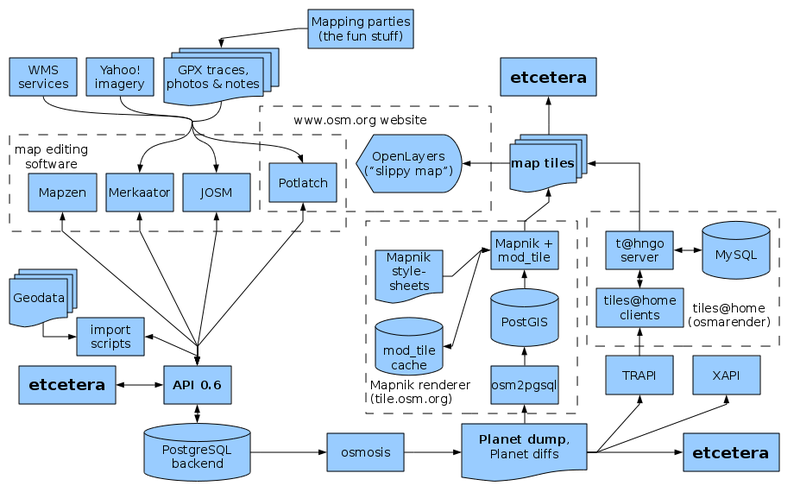
\includegraphics[width=0.85\textwidth]{images/800px-OSM_Components.png}
	\caption{Overview of OpenStreetMap's architecture.}
	\label{fig:osm-overview}
\scriptsize Source:\url{http://wiki.openstreetmap.org/w/images/1/15/OSM_Components.png} as of 2011 Apr 27th
\end{figure*}

To manage those datastructures, an infrastructure evolved encompassing multiple map editing tools, tile renderers, and data sources, as shown in Figure~\ref{fig:osm-overview}.

The data is stored in a relational database (PostgreSQL backend).
It can be accessed, queried and edited by using a REST API, which basically uses HTTP GET, PUT and DELETE requests with XML payload (similar to the example shown in Listing~\ref{lst:osc}).
The data is also published as complete dumps of the database in such an XML format on a weekly basis.
It currently accounts for more than 16GB of Bzip2 compressed data.
In minutely, hourly and daily intervals the project additionally publishes changesets, which can be used to synchronize a local deployment of the data with the OSM database.
The dumps as well as the changesets can be processed with the \emph{Osmosis} tool.

OpenStreetMap's community has build different authoring interfaces. These include the online editor \textit{Potlatch}, which is
implemented in Flash and accessible directly via the edit tab at the OSM map view, as well as the desktop applications \textit{JOSM}, \textit{Merkaartor} and \textit{Mapzen}. The editors use complementary external services and data such as \textit{Yahoo! satellite imagery} or \textit{Web Map Services} (WMS).
Additionally, users can upload GPS traces which serve as raw material for modelling the map.
Two different rendering services are offered for the rendering of raster maps on different zoom levels.
With \textit{Tiles@home}, the performance-intense rendering tasks are dispatched to idle machines of community members; thus achieving timeliness.
The \textit{Mapnik} renderer, in turn, operates on a central tile server and re-renders tiles only in certain intervals.

\begin{table*}[thb]
	\centering
		\begin{tabular}{lrrrr}
\textbf{Category} & \textbf{June 2009} & \textbf{April 2010} & \textbf{May 2011} & \textbf{Growth (past two years)} \\
\hline
Users (Thousands)	& 127 & 261 & 397 & + 213\% \\
Uploaded GPS points	(Millions) & 915 & 1500 & 2298 & + 151\% \\
Nodes (Millions)	& 374 & 600 & 1073 & + 187\% \\
Ways (Millions)	& 30 & 48 & 92 & + 207\% \\
% Relations	& 136,245 & ~300 & 6\% \\			
		\end{tabular}
% Quellen:
% 2009: http://jens-lehmann.org/files/2009/linkedgeodata_iswc.pdf
% 2010: http://aksw.org/files/claus_stadler__linkedgeodata__semantisch_vernetzte_geodaten.pdf
% 2011 (aktuell): http://www.openstreetmap.org/stats/data_stats.html
	\caption{OpenStreetMap statistics 2009 - 2011.\\(Obtained from \url{http://www.openstreetmap.org/stats/data_stats.html} at the specified months.)}
	\label{tab:OSMStatistics}
\end{table*}

Since the use of tags and values is not restricted, but governed by an agile community process, it is important to obtain an overview on emerging tags and tag values possibly specific to a certain region.
Services such as TagWatch\footnote{\url{http://tagwatch.stoecker.eu/}} periodically compute tag statistics for different areas.
In order for the data to be machine interpretable, as for instance for map rendering, contributors must follow certain editing standards and conventions\footnote{\url{http://wiki.openstreetmap.org/wiki/Map_Features}}.

Currently, OSM is in the process of switching from the Creative Commons CC-BY-SA license to the Open Database License\footnote{\url{http://www.opendatacommons.org/licenses/odbl/}}.
The term \textit{Volunteered Geographic Information} (VGI) was coined~\cite{michael2007citizens} for the harnessing of tools to create, assemble, and disseminate geographic data provided voluntarily by individuals -- with OSM being a driving force behind VGI.
% In any case, the data is freely available and is published as weekly full dumps. % Jens: wurde schon vorher gesagt
%Furthermore, changesets are provided on a minutely, hourly, and daily basis. % Jens: wurde schon vorher gesagt
% These datasets form the basis for LinkedGeoData.

The growth of the OpenStreetMap data has been enormous (cf. Table~\ref{tab:OSMStatistics}):
Since the founding in July 2004 until now, more than one billion nodes, about 90 million ways and close to 1 million relations have been contributed by the users\footnote{\url{http://www.openstreetmap.org/stats/data_stats.html}, retrieved 2011 May 2nd}.
Some of the data was imported form public domain datasources such as TIGER\footnote{\url{http://www.census.gov/geo/www/tiger}} for US, AND Automotive Navigation Data\footnote{\url{http://www.and.com/}} for The Netherlands, and GeoBase data from the Canadian government\footnote{\url{http://www.geobase.ca}}.

%\section{LinkedGeoData Overview}
\section{Architecture}
\label{sec:architecture}

The goal of the LinkedGeoData the project is to contribute rich, open, and integrated geographical data to the Semantic Web using OpenStreetMap as its base.
This is analogous to the well known DBpedia project, which follows a similar approach based on Wikipedia.
The necessary work for reaching this goal comprises the conversion of OSM data to RDF, the interlinking with other knowledge bases, the dissemination of the resulting data, and keeping the datasets up-to-date.
In this section, we give an overview of the LinkedGeoData architecture, followed by explanations of the details of the involved components in the next sections.

\begin{figure*}[htbp]
	\centering
%		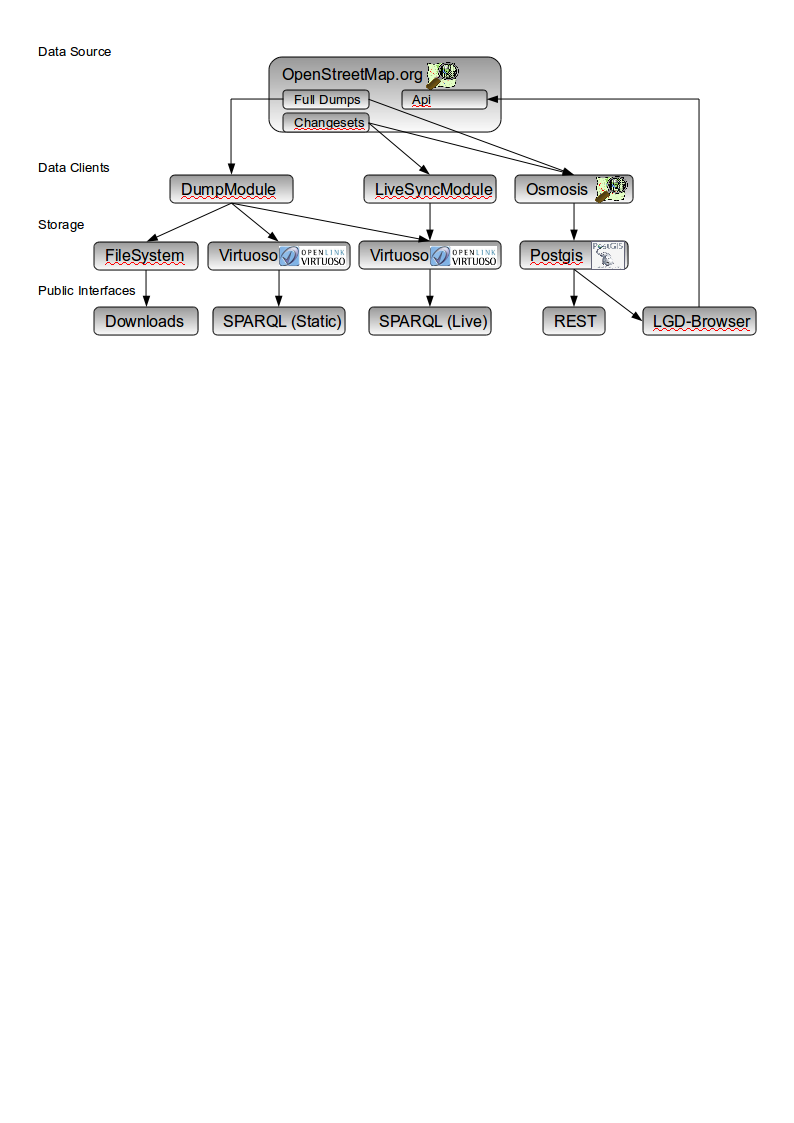
\includegraphics[width=\textwidth]{images/Architecture.png}
		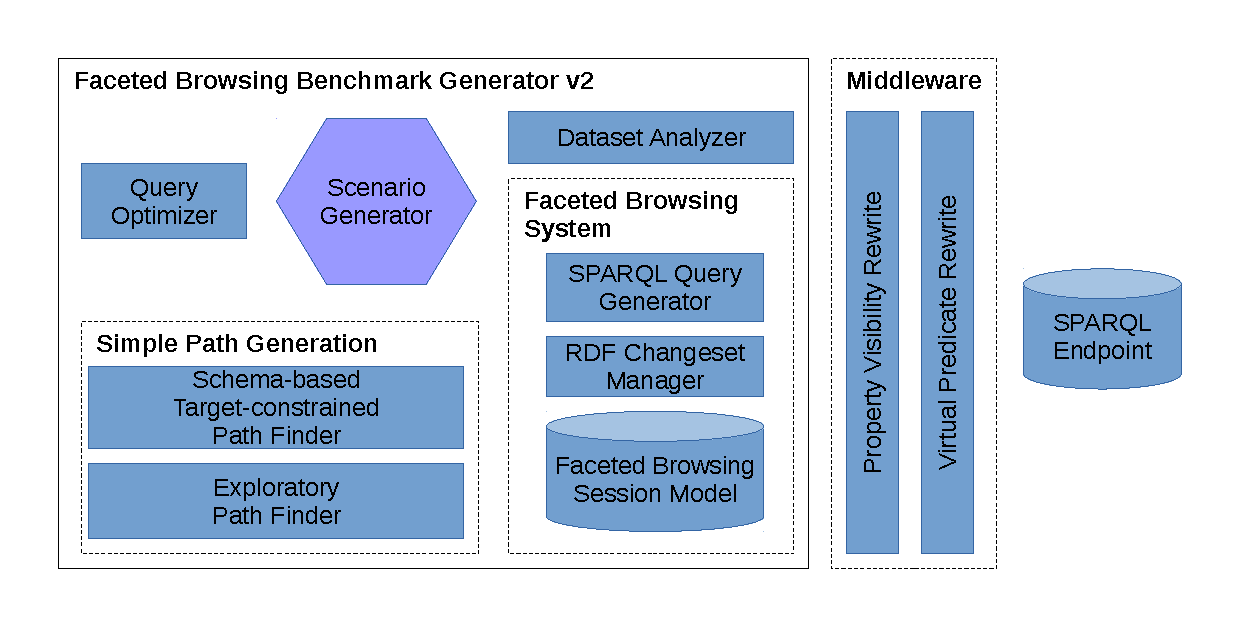
\includegraphics[width=0.85\textwidth]{images/Architecture.pdf}
	\caption{Overview of LinkedGeoData's architecture.}
	\label{fig:lgd-architecture}
\end{figure*}

%\subsection{Architecture}
The architecture of LinkedGeoData is illustrated in Figure~\ref{fig:lgd-architecture}.
It shows that the data from OpenStreetMap is processed on different routes:
The \emph{LGD Dump Module} converts an OSM planet file to RDF and loads the data
into a triple store. This data is then available via the
\emph{static SPARQL endpoint}.  A copy of that triple store serves as the initial basis
for the \emph{live SPARQL endpoint}.   
The \emph{LGD Live Sync Module} downloads minutely changesets from OpenStreetMap, and computes corresponding changesets on the RDF level in order to update that
triple store accordingly. 
By publishing these RDF changesets (see Section~\ref{sec:changeset-formats}), we enable data consumers to sync their own triple store with ours. Note, that not all OSM entities are loaded into the SPARQL endpoints due to performance reasons.
We offer SPARQL endpoints for the static and live version, because some use cases require up-to-date information whereas for others, it is more suitable that queries yield the same result over a longer period of time, e.g.~due to caching mechanisms.

For data access LinkedGeoData offers downloads, a REST API interface, Linked Data, and SPARQL endpoints.
The \emph{REST API} provides limited query capabilities for RDFized data
about \emph{all} nodes and ways of OpenStreetMap (relations are currently not
supported). It draws its data from a local replica of the OpenStreetMap PostGIS database.
The OpenStreetMap community developed a tool named 
\emph{Osmosis}\footnote{\url{http://wiki.openstreetmap.org/wiki/Osmosis}}, which
supports setting up such a database from a \textit{planet file} and applying
changesets to it. 
In future work, we aim for stronger support of spatial SPARQL queries by exposing PostGIS features via SPARQL.

% Jens: In obigen Text integriert. 
%The live SPARQL endpoint is synchronized with minutely updates from OSM, whereas the static one will contain all the data of the most recent LinkedGeoData release. Therefore, use cases which require up-to-date information as well as use cases where it is desirable for queries to yield the same results for a longer time span can be supported.
%Also, the static dump is more easy to set up from the downloads.
%Examples for uses of the live endpoint are the observation of an area in the
%search for new amenities or doing an evaluation on a particular area.

\section{RDF Mapping}
\label{sec:rdf_mapping}

In this section, we explain our approach to the generation of RDF triples from OpenStreetMap entities. 
Recall that all such OSM entities have a numeric ID and carry
information in form of values for predefined attributes and sets of tags.
The values for the predefined attributes, such as the version, the contributing
user, and timestamp are static and can also be seen as tags.

We generate URIs for nodes and ways according to the pattern
\verb=lgd:node<id>= and \verb=lgd:way<id>=, respectively.\footnote{See Appendix~\ref{sec:prefixes} for prefix declarations.} The resource
corresponding to a way's list of nodes is \verb=lgd:way<id>/nodes=.

These URIs are non-information resources, i.e. they represent
real-word entities. As such, stating that a resource corresponding to a pub
was created by a building company would be correct, however stating that it was
created with the map editor ``JOSM'' would be wrong.
In general, there are two possible solutions to permit both kinds of
statements: a) introduce distinct URIs for each of the two different
meanings, b) make use of annotation properties, which are intended for this purpose and do not have any logical implications. 
We chose the latter approach, because it avoids doubling the number of resources and keeps the data simple.
% for two reasons: Firstly it avoids doubling the number of resources, and secondly it keeps the data more simple. \todo{J

Our tag mapping approach is based on the assumption that each tag can be mapped in isolation, i.e.~without taking other possibly existing tags into account.
For example, entities with the tag \texttt{(amenity, school)} become instances of \texttt{lgdo:School}. 
Note, that this approach does not support more complex rules such as mapping all entities having both tags \texttt{(amenity, place\_of\_worship)} and \texttt{(religion, christian)} to e.g. \texttt{lgdo:Church}.
Therefore, the generated RDF structures are very close to the structure in OpenStreetMap.

We now specify the mapping process.
A \emph{tag mapper} is an object for generating RDF from tags.
It consists of a \emph{tag pattern} that specifies what tags to match,
and a \emph{transformation function} for generating the RDF.

Tag patterns can 1) match a specific key-value pair, such as \texttt{(amenity, school)}, 2) match all tags with a certain key (regardless of the values), e.g. \texttt{(tourism, *)}, or 3) match every tag. 
More specific patterns take precedence, e.g.~a matching pattern in category 1 overwrites matching patterns in category 2 and 3.
% A more concrete pattern implicitly takes precedence over less concrete patterns. This means, that the rule that matches every tag is only applied if no other rule matches.

We implemented the following four tag mappers:
\begin{itemize}
  \item \emph{Resource}: Maps a tag to a specific property and
  object, where both must be URIs. Therefore it can be used for mapping to
  both object properties and classes. In the latter case the property
  has to be set to \texttt{rdf:type}.
  Examples are \emph{(religion, christian)} and \emph{(amenity, school)} which
  are mapped to \emph{lgdo:religion lgdo:christian} and
  \emph{rdf:type lgdo:School}, respectively.
  \item \emph{Text}: Treats a tag's value as a plain literal. For example
  \emph{(note, nice view)}.
  \item \emph{Datatype}: Interpret a value e.g. \emph{(seats, 4)} with regard
  to a specific datatype.
  \item \emph{Language}: A mapper for tags whose key contains a
  language, such as \texttt{name:en}.
\end{itemize}

All of these mappings are implemented as Java classes, whose instances are
configured with an XML snippet. Listing~\ref{lst:tag-mapping} shows an example
of a configuration of a resource tag mapper that is interpreted as
follows: The 'simple' in the name reflects our limitation that tags are being
mapped in isolation. The mapping rule is applied to every entity that has a tag
matching the pattern \texttt{(religion,*)}.  The element \emph{objectAsPrefix} 
controls whether a tag's value should be appended to the value given as the object.
So in this case, a tag, such as \texttt{(religion, hindi)}, is mapped to the
predicate \texttt{lgdo:religion} and object \texttt{lgdo:hindi}.
The element \emph{describesOSMEntity} specifies whether the resulting RDF
describes a real world entity's representation on OpenStreetMap or the entity
itself. Therefore, it determines whether a mapping's property
should become an instance of \emph{owl:AnnotationProperty}.

The text- and datatype tag mappers are both similar to the resource tag
mapper, except that they map tag values to objects that are plain or typed
literals, respectively. Therefore the language and datatype of these mappers can
be set to a constant in their configuration.


The language tag mapper is used for mapping tag values to plain
literals with language tags inferred from the tags' keys. For instance
\emph{(name:en, Vienna)} would become \emph{(rdfs:label, ``Vienna''@en)}.
The key of its tag-pattern must be a regular expression containing a group for
matching the language, such as \verb=name:([^:]+)=. Every match for this
group is then cross checked against a list of known languages. This avoids for
example matching 'alt' as a language from the key
\emph{name:alt} for alternative names.

\begin{scriptsize}
\begin{lstlisting}[label=lst:tag-mapping, language=XML, caption=Example of a mapping declaration.]
<SimpleResourceTagMapper>
  <property>
    http://linkedgeodata.org/ontology/religion
  </property>
  <tagPattern>
    <key>religion</key>
  </tagPattern>
  <describesOSMEntity>false</describesOSMEntity>
  <objectAsPrefix>true</objectAsPrefix>
  <object>
    http://linkedgeodata.org/ontology/
  </object>
</SimpleResourceTagMapper>
\end{lstlisting}
\end{scriptsize}

This approach makes it possible to add new mappings that require more complex
processing easy. For example, a future tag mapper could extract the values of
\texttt{opening\_hours} tags (used ~60K times on nodes) and generate RDF in the
\textit{Good Relations}\footnote{\url{http://www.heppnetz.de/projects/goodrelations/}} vocabulary.

\subsection{The LinkedGeoData Ontology}
Based on the OpenStreetMap tags, we derived a lightweight OWL
ontology\footnote{The complete ontology is available at \url{http://linkedgeodata.org/ontology/}}.
A depiction of an excerpt in shown
in Figure~\ref{fig:ontology-excerpt}.
\begin{figure}[htbp]
	\centering
%		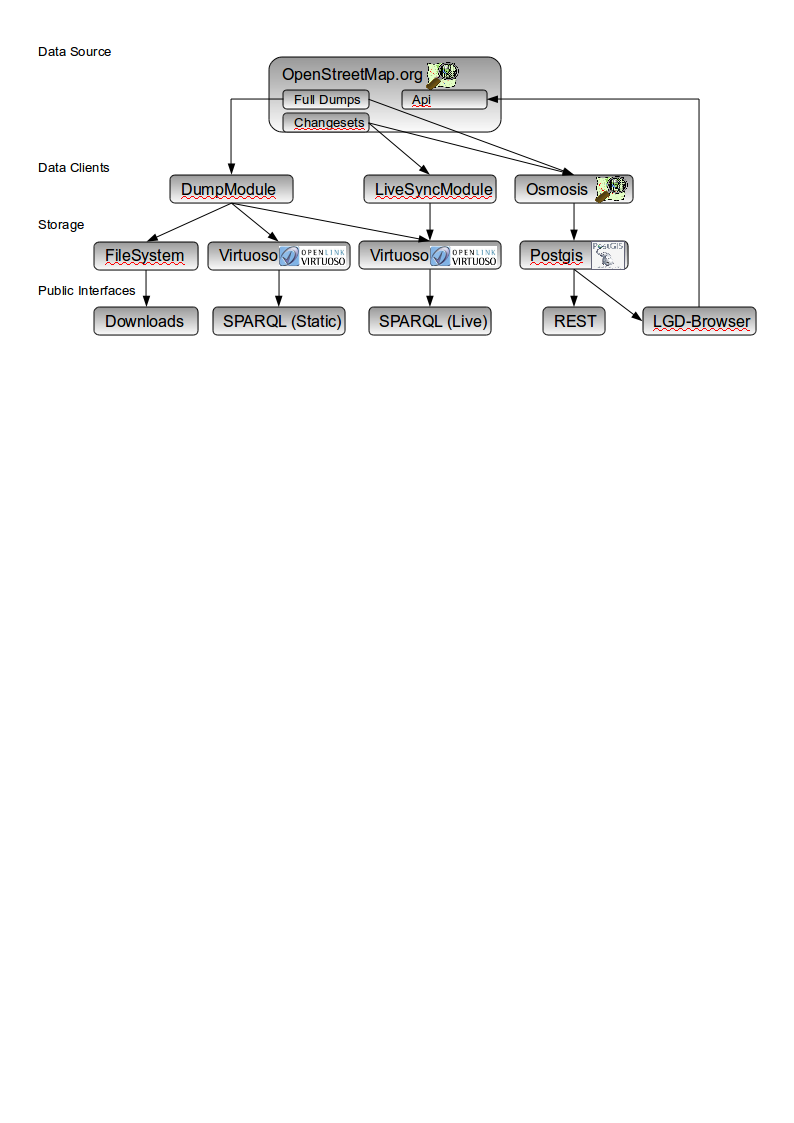
\includegraphics[width=\textwidth]{images/Architecture.png}
		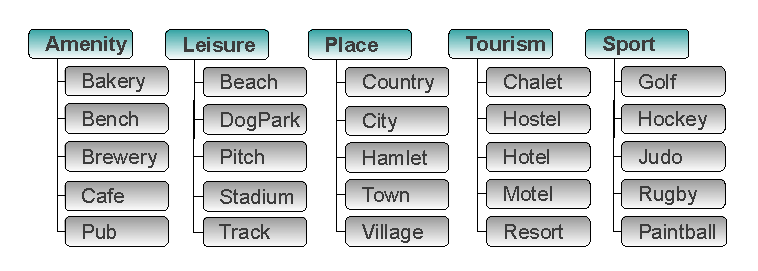
\includegraphics[width=0.5\textwidth]{images/OntologyExcerpt.pdf}
	\caption{An excerpt of the LinkedGeoData ontology.
	More classes and subclasses exist in the actual version.}
	\label{fig:ontology-excerpt}
\end{figure}
%\footnote{The full ontology is available at
%\url{http://linkedgeodata.org/ontology/}}

The process of creating it is explained as follows:
Subclass relationships are inferred from resource tag mapper configurations: If
there are two tag patterns for \emph{(tag1, tag2)} and \emph{(tag1, *)}, which
use the \verb|rdf:type| property, then the object of the first tag pattern
becomes a subclass of the second tag pattern. For example,
Listing~\ref{lst:tag-mapping-subclass} shows an example of such tag mappings
for the \emph{(amenity, restaurant)} and \emph{(amenity, *)} tag patterns.

%\todo{Jens: Habe es in zwei Saetze zerlegt und vereinfacht. Bitte pruefen, ob es dennoch korrekt ist. Inbesondere koennte man erwaehnen, warum das \emph{(amenity, *)} ueberhaupt notwendig ist, d.h. warum es nicht reicht das tag2 auf eine Klasse gemappt wird.}
% If for a specific tag-pattern, such as \emph{(amenity, restaurant)}, there exists less specific one, such as \emph{(amenity, *)}, and both corresponding mapping rules map entities to instances of classes, such as \emph{Amenity} and \emph{Restaurant}, then the class of of the specific tag-pattern becomes a sub-class of the general one. In this example we would infer that \emph{Restaurant} is a subclass of \emph{Amenity}.

\begin{scriptsize}
\begin{lstlisting}[label=lst:tag-mapping-subclass, language=XML, caption=Subclass relationship example.]
<SimpleResourceTagMapper>
  <property>rdf:type</property>
  <tagPattern>
    <key>amenity</key>
  </tagPattern>
  <describesOSMEntity>false</describesOSMEntity>
  <objectAsPrefix>false</objectAsPrefix>
  <object>
    http://linkedgeodata.org/ontology/Amenity
  </object>
</SimpleResourceTagMapper>
<SimpleResourceTagMapper>
  <property>rdf:type</property>
  <tagPattern>
    <key>amenity</key>
    <value>restaurant</value>
  </tagPattern>
  <describesOSMEntity>false</describesOSMEntity>
  <objectAsPrefix>false</objectAsPrefix>
  <object>
    http://linkedgeodata.org/ontology/Restaurant
  </object>
</SimpleResourceTagMapper>
\end{lstlisting}
\end{scriptsize}

In order to determine datatype properties, we scanned all OSM tags for those that had keys for which the majority of values could be parsed as boolean, integer, and float datatype values. 
In order to deal with dirtiness in tag usage, we applied the following two criteria on the relative and absolute error rate:
\begin{itemize}
  \item At least 99\% of a key's values must succeed to parse.
  \item The absolute number of errors must not exceed 5000.
\end{itemize}
The most specific datatype meeting these criteria then became the range of the key's corresponding property. 
If a datatype was determined, all invalid values were omitted in the RDF output.

Object properties were identified as follows:
Intuitively, tags that might be suitable for being mapped to object properties meet the condition, that a low number of distinct values covers most its uses. 
However, this heuristic only serves as an indicator for tag candidates, as the final choice may be subjective.
For instance, only 7 distinct values for the key \emph{note:ja} are used in more than 99\% of almost 3.5mio tags. 
However, since the tag corresponds to a note, we considered a datatype property to be the right choice.
%\todo{Beispiel fuer object property angeben.}
An example for an object property is \emph{lgdo:religion}, which links to
resources in the \emph{lgdo} namespace, such as \emph{christian}, \emph{muslim},
and \emph{buddhist}.
Another example is \emph{lgdo:wheelchair}, which specifies the extent of
wheelchair accessibility, using resources mainly corresponding to the
values \emph{yes}, \emph{no}, \emph{limited}, and \emph{unknown}.
Using those heuristics, we could generate seed mappings for OpenStreetMap, which were then manually reviewed and refined.


\subsection{Multilingual labels and icons}
The OpenStreetMap community conducts various internationalization efforts, such as for
their website, their map editing tools, and their search engine.
Some of these efforts are coordinated on \emph{TranslateWiki}, which describes
itself as ``a localisation platform for translation communities, language
communities, and free and open source
projects.''\footnote{\url{http://translatewiki.net}} Essentially, this wiki
enables contributors to assign texts in multiple languages to keys.
The group \emph{OpenStreetMap - Website} defines 1441 keys, and has a 100\%
translation coverage for 13 languages and 12 more languages with a coverage of
more than 90\%\footnote{\url{http://translatewiki.net/wiki/Translating:OpenStreetMap/stats/trunk} retrieved 5th May 2011.}.
They keys with the prefix \emph{geocoder.search\_osm\_nominatim.prefix}
correspond to human readable representations of individual tags, and as such
form a rich, multilingual, and high quality source of labels for classes,
properties, and instances, which we integrated into the LinkedGeoData ontology.

These labels could serve as a basis for answering queries posed in different
languages: For a query such as ``Bakeries in Munich'' and its German
equivalent ``B\"{a}ckereien in M\"{u}nchen'', the search words could be mapped
to corresponding classes and instances from the LinkedGeoData knowledge
base.
A system already capable of processing such types of queries is described
in~\cite{spirit}.


As for icons, there exists a \textit{CC-0} licensed collection of 307 SVG map
icons (of which 47 icons are alternative versions) from SJJB
Management.\footnote{\url{http://www.sjjb.co.uk/mapicons/} retrieved 6th April 2011}
Currently the LinkedGeoData ontology associates 90 of them with classes,
using the annotation property \emph{lgdo:schemaIcon}.
The icons themselves are re-published on our server. 
They simplify the creation of visually appealing LGD based applications and mashups.

\section{Data Access}
\label{sec:data_access}

As briefly mentioned in Section~\ref{sec:architecture}, we provide several ways to access LinkedGeoData:
\begin{itemize}
 \item dataset downloads (HTML download table\footnote{\url{http://linkedgeodata.org/Datasets}} and actual files\footnote{\url{http://downloads.linkedgeodata.org}}), including live sync changesets relative to the latest release\footnote{\url{http://downloads.linkedgeodata.org/releases/latest/changesets/}} (explained in Section~\ref{sec:synchronization})
 \item a static SPARQL endpoint\footnote{\url{http://linkedgeodata.org/sparql}}
 \item a live SPARQL endpoint\footnote{\url{http://live.linkedgeodata.org/sparql}}
 \item Linked Data via 303 content negotation (RDF/XML, Turtle, N-Triples, HTML formats supported)
 \item a REST API
\end{itemize}

We first show an example data excerpt and then explain the REST API.

\subsection{Data example}
In Listing~\ref{lst:lgd-dataset-example}, we give a brief example on how the data in LinkedGeoData looks like.
The whole type hierarchy is already inferred, as it is being done in DBpedia, i.e.~\verb|rdf:type| relations to all super classes are asserted.
The \emph{lgdo:directType} property was added on request in order for applications to easily determine the most specific types of instances.
For every way, there exists a triple that contains the positions of all nodes.
For open and closed ways the predicates are \emph{georss:linestring} and \emph{georss:polygon}, respectively.
Note that this interpretation is not always correct, as in the general case closed ways have to be interpreted in the context of the ways' tags in order to determine whether the enclosed area counts to the way or not.
All nodes belonging to a way are kept in an RDF sequence.
In the SPARQL endpoints, geographical coordinates are represented as point geometries that are typed with \emph{virtrdf:Geometry}.
OpenLink's Virtuoso\footnote{\url{http://virtuoso.openlinksw.com}} enterprise
edition database system automatically indexes such points in an R-tree.

\begin{scriptsize}
\begin{lstlisting}[label=lst:lgd-dataset-example, language=ttl, caption=Example dataset in Turtle syntax.]
lgd:way4009992
  a            lgdo:Tennis, lgdo:Sport, lgdo:Way;
  lgdo:directType  lgdo:Tennis;
  lgdo:contributor lgd:user2274;
  lgdo:hasNodes    <http://.../way4009992/nodes>;
  georss:polygon  "52.1523857 -1.026259
                     52.1522675 -1.0264068 ..." .
<http://.../way4009992/nodes>
  a       rdf:Seq;
  rdf:_1  lgd:node21179607;
  rdf:_2  lgd:node21179608;
  ... .
lgd:node21179607 geo:geometry
  "POINT(-1.02626 52.1524)"^^virtrdf:Geometry
\end{lstlisting}
\end{scriptsize}

\subsection{The REST API}

\begin{figure}[htbp]
	\centering
%		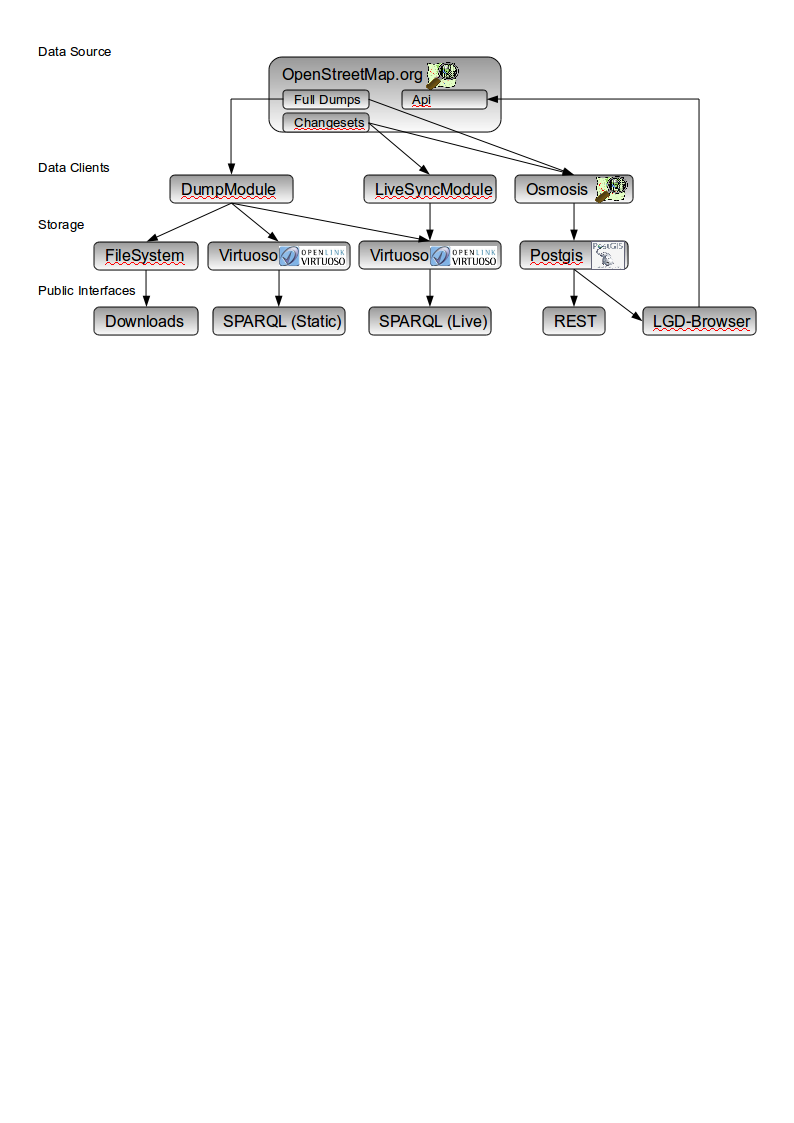
\includegraphics[width=\textwidth]{images/Architecture.png}
		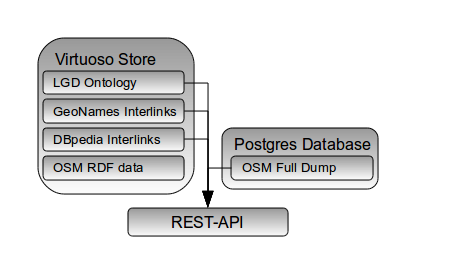
\includegraphics[width=0.4\textwidth]{images/RestArchitecture.png}
	\caption{Data Sources of the REST API.}
	\label{fig:rest-api-architecture}
\end{figure}

%In this section we introduce the LinkedGeoData REST API.
The LinkedGeoData REST API gives access to all of OpenStreetMap's nodes and ways.
It offers a set of methods that all have in common that they return RDF for responses. 
Each call to the REST API can be combined with content negotiation to format these responses as RDF/XML, N-Triples, or Turtle.
The API is backed by two things: on the one hand there is a PostGIS database
that is loaded with an OSM planet file and which is updated with minutely OSM changesets. On the other hand, the data for the ontology and interlinking is drawn from the SPARQL endpoints, as depicted in Figure~\ref{fig:rest-api-architecture}.

\begin{table*}[htb]
\begin{tabular}{ll}
\toprule
URLs relative to \url{http://linkedgeodata.org/triplify/near/} & Description \\
(General syntax and specific example) \\
\midrule
% Jens: würde ich rausnehmen, da als Linked Data im Text beschrieben
%\url{ontology} & Retrieves the whole ontology \\
%\url{node264695865} & Retrieves information about a specific node. \\
%\url{way4564184} & Same for ways \\
\url{<latmin>-<latmax>,<lonmin>-<lonmax>} & Resources located in the given rectangle. \\
\url{51.02-51.04,13.72-13.74}  \\
\url{<lat>,<lon>/<radius>} & Resources located in specified radius in meters from the given point. \\
\url{51.02-51.04/1000}  \\
\url{<lat>,<lon>/<radius>/class/<classname>} & Resources in specified radius belonging to the given class. \\
\url{51.033333,13.733333/1000/class/PlaceOfWorship} \\
\url{<lat>,<lon>/<radius>/class/} & Resources in specified radius, belonging to the given class with a \\
\url{<classname>/label/<lang>/contains/<label>} & label in the specified language containing a specific string. \\
\url{.../class/Amenity/label/en/contains/flower} \\ 
%\url{near/.../class/Shop/label/contains/any/flower} & Same as above,
%additionally instances must be of class \texttt{lgdo:Shop} \\
% & and their label must contain the substring ``flower'' in any language.
\bottomrule
\end{tabular}
\caption{Excerpt of the methods supported by the LGD REST API.}
\label{tab:rest-api-methods}
\end{table*}

An excerpt of the available methods is given in Table~\ref{tab:rest-api-methods}.
In general, the REST API returns a set of spatial entities along with their RDF descriptions, which can be filtered in numerous ways:
\begin{itemize}
 \item by area: Either a circular or rectangular area can be selected via WGS84 coordinates.
 \item by class: Returned resources can be restricted to a single LinkedGeoData class.
 \item by name (\verb|rdfs:label|): It can be set whether returned points should contain or start with a certain string. Furthermore, it can be specified whether name search should be case sensitive and whether only names with a particular language tag should be considered.
\end{itemize}
Using area and label search combined with class restrictions were the most requested features in applications, which is why we provide them in the REST interface.
The main purpose of the REST API is to lower the entry barrier for data consumers and to internally optimise the performance of the most commonly used queries.

\section{Interlinking}
\label{sec:interlinking}

% Jens: Habe das in den Anhang verschoben.
\begin{comment}
\tymin20pt
\begin{table}[ht]\label{tab:prefixes}
\begin{tabulary}{0.5\textwidth}{LL}
\toprule
prefix	&URL\\
\midrule
%lgd	&\url{http://linkedgeodata.org/}\\
lgdo	&\url{http://linkedgeodata.org/ontology/}\\
%lgdt	&\url{http://linkedgeodata.org/triplify/}\\
gn	&\url{http://www.geonames.org/ontology\#}\\
wgs84 	&\url{http://www.w3.org/2003/01/geo/wgs84_pos\#}\\ 
foa	&\url{http://www.fao.org/countryprofiles/geoinfo/geopolitical/resource/}\\
\bottomrule
\end{tabulary}
\caption{The prefixes used in this section}
\end{table}
\end{comment}

In this section, the interlinking between \emph{LinkedGeoData},
\emph{DBpedia}, \emph{GeoNames} and the
\emph{Food and Agriculture Organization of the United Nations (FOA)} is
described.
In all cases, we first manually aligned the classes of these
knowledge bases with classes from LinkedGeoData on an best effort basis.
The interlinking is then done on a per-class basis, where all instances of a set
of classes of LGD are matched with all instances of a set of classes of another data source using labels and spatial information. As an example, cities in LGD
and DBpedia are matched between all instances of \nolinkurl{lgdo:City}, \nolinkurl{lgdo:Town}, \nolinkurl{lgdo:Village} and
\nolinkurl{lgdo:Hamlet} on one side and \nolinkurl{dbo:Settlement} on the other.
The interlinking is performed using the tools SILK~\cite{silk} and
LIMES~\cite{limes}, which use the static SPARQL endpoint as the backend. As
Virtuoso's index support for geometries is limited to points, we needed to constrain the interlinking to
LinkedGeoData nodes. An overview of triple stores supporting complex
geometries is given in Section~\ref{sec:geo-semantic-web}.

%In contrast, a LinkedGeoData way does not have a position itself, but has a
%potentially high number of nodes, each of which has a WGS84 position.
It should be noted, that many ways in OpenStreetMap have reference
points, e.g.~characteristic points for a given way. Those reference points
are not necessarily located in the geometric center of a way, but represent
a typical point by OSM community consensus.

%instead may contain millions of points describing the path 
%or outline of a geographical feature and is thus unsuitable for this kind of matching.
\iffalse %rausgenommen, weil das schon in der Statistik drin ist
\begin{table}[hb]
\begin{tabular}{lr}
\toprule
class				&number of instances\\
\midrule
City $\cup$ Town $\cup$ Village $\cup$ Hamlet 	&\val{818893}\\
%City $\cup$ Town $\cup$ Village 		&\val{544890}\\
School						&\val{331242}\\
Building					&\val{257893}\\
Park 						&\val{151833}\\
Peak						&\val{148580}\\
Waterway 					&\val{90455}\\
Island						&\val{51472}\\
River 						&\val{2651}\\
Country 					&\val{235}\\
\bottomrule
\end{tabular}
\caption{Some LinkedGeoDatas classes, not counting transitive membership.}
\label{tab:geonames-featureclasses}
\end{table}
\fi

For each class-mapping, a link specification is created and executed using the \emph{Silk Link Discovery Framework} \cite{silk}.
The link specs usually include a metric, which is a linear classifier depending on the labels and the geographic distance,
which can be calculated from the values of \nolinkurl{wgs84:lat} and \nolinkurl{wgs84:long} properties which are provided by all considered data sources.
By combining classification, naming and spatial features, we are able to obtain very precise interlinking heuristics as shown later.

We used the following matching criterion, which we explain in detail below:
\[\frac{2}{3} s(a,b) + \frac{1}{3} g_c(a,b) > 0.95\]

\begin{itemize}
 \item $a$ and $b$ are the resources to be compared
 \item $s(a,b)$ is a the \emph{Jaro-Winkler distance}~\cite{WIN99}, between the
 labels of $a$ and $b$. If there are multiple labels, the pair with the maximum score is chosen, ignoring the language-tag.
While this could cause false links in the special case that the label of a
resource in one language is very similar to the label of a resource in a
different language, this type of error was not found in our evaluation.
%between pair of different geographical features $A$ and $B$, where the name of one in one language
%is very similar to name of the other in another language, this particular error was not found in our evaluation.
An advantage of this approach is that it works for several languages even if the proper language tags are actually missing.
% On the other hand, this approach can make use of the many labels without a language tag and is simple to implement in \emph{SILK}.
 \item $c$ is the maximum distance that two points describing the same object are reasonably expected to differ.
While a good value for $c$ is easily chosen in some cases (a shop does not span more than a few hundred meters), it is nontrivial in cases of large variances
in size such as in cities, mountains or islands.
The value of $c$ varies greatly between classes and is explained by the choice of reference points, which can differ in each of the considered knowledge bases.
 \item $g_c(a,b) =
\begin{cases}
0 & d > c \\
1/(1+e^{-12d'+6}) & otherwise
\end{cases}$
In this formula, $d$ is the distance between $a$ and $b$. The distance is approximated by the \emph{haversine formula}, which uses a spherical model of the earth.
We then define $d' = 1 - d/c$ which is a linear function with a value of zero at distance $d=c$ and one for $d=0$.
In order to not punish a slight discrepancy between two points as much as a linear function would, $d'$ is not used directly.
Instead, we employ a scaled logistic curve. The remaining parameters are adjusted such that two objects at distance $c$ with exactly the same labels almost exactly matches the threshold of 0.95 in the formula above, which is the intended meaning of the parameter $c$.
\end{itemize}

%Because of the chosen threshold of \val{0.95} however, two entities with a distance of exactly $c$ would not be considered a match even 
%if their labels were exactly equal.
%This is alleviated by using $c' = 4c$ instead of $c$,
%because in this case $d' = 1 - \frac{c}{4c} = \frac{3}{4}$ and $1/(1+e^{-12\frac{3}{4}+6}) \approx \val{0.952}$.
%This means that as long as the string similarity value is above $\val{0.95}$, a distance of $c$ is guaranteed to be a match.

%\footnotetext{$2/3+1/3*x = \val{0.95}$}
\iffalse
2/3+1/3*x = 0.95
1/3 x = 0.95 -2/3
x = 0.95*3-2 = 3-2-0.05*3 = 1 0.15 = 0.85
\fi
\subsection{Interlinking with DBpedia}
Since the initial interlinking between LinkedGeoData and DBpedia as described in \cite{linkedgeodata} in 2009, both knowledge bases have
grown and changed significantly, resulting in the need of a new interlinking as well as an exhaustive re-evaluation of the quality of the interlinks.
Table~\ref{tab:linkedgeodata-dbpedia-matching} shows the created class-mappings and the size of the linksets and their estimated precisions.
The links were manually evaluated with a random sample of 250 instances each. In cases where the number of links is smaller
than or only slightly higher than 250 as in the case of the universities, all of the instances were evaluated.
\tymin=1pt
%\tymax=100pt
\begin{table}[ht]
\caption{LinkedGeoData-DBpedia linksets.}
\label{tab:linkedgeodata-dbpedia-matching}
\begin{threeparttable}
\begin{tabulary}{0.502\textwidth}{LRLRRRR}
\toprule
DBpedia	class		&instances	&LGD equivalent		&c in km			&nodes		&links		&precision\\
\midrule
Airport			&9520		&Aerodrome		&2.5	&43734	&8404	&1.0\\
Settlement 		&239630		&several\tnote{1}			&0.1	&620387	&88377	&1.0\\
Country			&2505\tnote{2}	&Country		&1000	&231	&222	&0.991\\
%x			&	&				&				&		&\\
University		&11607	&University			&2.5	&17715	&268	&1.0\\
Stadium			&5539	&Stadium			&1	&13001	&133	&1.0\\
School			&22686	&School				&1	&262566	&2470	&1.0\\
Island			&2371	&Island				&100	&31121	&449	&1.0\\
Mountain		&8742	&Peak				&100	&177702	&3258	&0.992\\
\midrule
Overall			&302600	&				&			&1166457	&103581	&0.966\\
% Jens: too few links
% Lake			&\val{8221}	&Water				&\valunit{25}{km}			&\val{311}		&\val{0}	&\val{0.0}\\
% Jens: too few links
%River			&\val{18526}	&Waterway $\cup$ River		&\valunit{250}{km}			&\val{93106}		&\val{8}	&\val{1.0}\\
% old with valunit:
\iffalse
DBpedia	class		&instances	&LGD equivalent	&c in km			&nodes		&links		&precision\\
\midrule
Airport			&\val{9520}	&Aerodrome			&\val{2.5}	&\val{43734}	&\val{8404}	&\val{1.0}\\
Settlement 		&\val{239630}	&City $\cup$ Suburb $\cup$ Town $\cup$ Village
									&\val{0.1}	&\val{620387}	&\val{88377}	&\val{1.0}\\
Country			&\val{2505}\tnote{1}	&Country		&\val{1000}	&\val{231}	&\val{222}	&\val{0.991}\\
%x			&\val{}	&				&\val{}				&\val{}		&\val{}\\
University		&\val{11607}	&University			&\val{2.5}	&\val{17715}	&\val{268}	&\val{1.0}\\
Stadium			&\val{5539}	&Stadium			&\val{1}	&\val{13001}	&\val{133}	&\val{1.0}\\
School			&\val{22686}	&School				&\val{1}	&\val{262566}	&\val{2470}	&\val{1.0}\\
Island			&\val{2371}	&Island				&\val{100}	&\val{31121}	&\val{449}	&\val{1.0}\\
Mountain		&\val{8742}	&Peak				&\val{100}	&\val{177702}	&\val{3258}	&\val{0.992}\\
\fi
\bottomrule
\end{tabulary}
\begin{tablenotes}
\item [1] City $\cup$ Suburb $\cup$ Town $\cup$ Village
\item [2] The large number of countries is caused by former countries like \emph{Republic of Texas} and \emph{Inca Empire}.
\end{tablenotes}
\end{threeparttable}
\end{table}

%TODO: Konrad - Kapitel schreiben
%
%DBpedia, GeoNames + möglichst weitere wie z.B. Flughafen Codes o.ä. verlinken => LinkedGeoData sollte als Hub im GeoDaten-Web erscheinen 
%TODO Claus: Schemalinks publizieren (es ist nicht notwending die wieder aus den instanzen rauszufinden (reading group seite))

\subsection{Interlinking with GeoNames}
The GeoNames database contains over 10 million geographical names and has 7.5 million unique features.
It integrates sources such as the \emph{National Geospatial-Intelligence Agency's} (\emph{NGA}) and the \emph{U.S. Board on Geographic Names}.
While at the time of this writing there is no official SPARQL endpoint yet, an RDF-dump and an ontology are available.
The ontology is very flat, with only two layers of disjunctive classes, where the superclasses are called \emph{feature classes} and the subclasses \emph{feature codes}.
The feature codes are very detailed, for example there are 97 feature codes for the feature type \nolinkurl{T} (\emph{Peak}).
Linking GeoNames with LinkedGeoData makes these detailed features available to
LinkedGeoData. In addition to the steps used for linking LinkedGeoData with DBpedia, the labels (which are represented by the properties \nolinkurl{gn:name} and \nolinkurl{gn:alternateName} in GeoNames) are first transformed by removing all occurrences of the name of class of the instances (e.g. \emph{``city''}). This increases the string similarity score for pairs like (``Fananu'', ``Fananu Island'').
Again, 250 links per class were evaluated and the results are shown in
Table~\ref{tab:linkedgeodata-geonames-matching}.

\tymax=140pt
\begin{table*}[ht]
\begin{threeparttable}
\caption{Matching classes and created links between LGD and Geonames.}
\label{tab:linkedgeodata-geonames-matching}
\begin{tabulary}{\textwidth}{LRLRRRR}
%\begin{tabulary}{\textwidth}{LLRLLR}
\toprule
GeoNames feature class or code				&number of features	&LinkedGeoData class	&c		&number of nodes	&links	&precision\\
\midrule
PCL $\cup$ PCLD $\cup$ PCLF $\cup$ PCLI $\cup$ PCLIX $\cup$ PCLS
						&\val{237}		&Country			&\valunit{1000}{km}		&\val{235}		&\val{218}	&\val{0.995}\\

PRK						&\val{71764}		&Park				&\valunit{5}{km}		&\val{151833}		&\val{55648}	&\val{0.992}\\
PPL $\cup$ PPLA $\cup$ PPLA2 $\cup$ PPLA3 $\cup$ PPLA4 $\cup$ PPLC $\cup$ PPLF $\cup$ PPLG $\cup$ PPLL $\cup$ PPLQ $\cup$ PPLR $\cup$ PPLS $\cup$ PPLW
						&\val{2821405}		&Hamlet $\cup$ Village $\cup$ Town $\cup$ City	
													&\valunit{100}{km}\tnote{1}		&\val{818893}		&\val{34907}		&\val{0.984}\\
%S						&\val{1554654}		&Building							&\val{257893}	&\val{}	&\val{}\\
%T\tnote{1}					&\val{1014431}		&Peak				&\valunit{100}{km}		&\val{148580}		&\val{236711}	&\val{0.518}\\
%ISL						&\val{28189}		&Island				&\valunit{400}{m}		&\val{51472}		&\val{37399}	&\val{0.631}\\
SCH						&\val{224217}		&School				&\valunit{1}{km}		&\val{340039}		&\val{168545}	&\val{1.0}\\
PRK						&\val{72130}		&Park				&\valunit{5}{km}		&\val{157862}		&\val{55648}	&\val{0.992}\\
%T						&\val{1015114}		&Peak	&\val{177727}	&\val{236711}	&\val{}\\
% commented out, because it is not evaluated
%STM $\cup$ STMM $\cup$ STMC $\cup$ STMSB $\cup$ STRT $\cup$ STMIX $\cup$ STMA $\cup$ STMS $\cup$ STMB $\cup$ STMH $\cup$ STMX $\cup$ STMD $\cup$ STMQ $\cup$ STMI
%						&\val{833870}	&River $\cup$ Waterway	&\val{3233409}	&\valunit{1000}{km}		&\val{47101}	&\val{?\tnote{2}}\\			
STDM						&\val{753}		&Stadium			&\valunit{1}{km}		&\val{13001}		&\val{24}	&\val{1.0}\\
FRM $\cup$ FRMQ $\cup$ FRMS $\cup$ FRMT		&\val{207171}		&Farm				&\valunit{6000}{m}		&\val{3834}		&\val{54}	&\val{1.0}\\
AIRH $\cup$ AIRP $\cup$ AIRQ $\cup$ AIRB $\cup$ AIRF	&\val{32449}	&Airport $\cup$ Aerodrome $\cup$ Aerialway $\cup$ Aeroway
													&\valunit{10}{km}		&\val{175006}		&\val{21552}	&\val{1.0}\\
% not enough links													
% PKLT						&\val{119}		&Parking			&\valunit{1}{km}		&\val{494787}		&\val{1}	&\val{1.0}\\
MALL $\cup$ MKT					&\val{18240}		&Supermarket $\cup$ Shop $\cup$ Mall		
													&\valunit{1}{km}		&\val{572833}		&\val{59}	&\val{0.949}\\
TMPL $\cup$ CH $\cup$ CTRR			&\val{231678}		&PlaceOfWorship			&\valunit{1}{km}		&\val{352673}		&\val{201318}	&\val{0.976}\\
REST						&\val{1195}		&Restaurant			&\valunit{1}{km}		&\val{167293}		&\val{55}	&\val{1.0}\\
% not enough links
% GRVE						&\val{561}		&GraveYard			&\valunit{5}{km}		&\val{134371}		&\val{1}	&\val{1}\\
% not enough links
% DPOF						&\val{23}		&Fuel				&\valunit{1}{km}		&\val{124296}		&\val{1}	&\val{1}\\
HTL						&\val{82876}		&TourismHotel			&\valunit{200}{km}		&\val{63516}		&\val{2214}	&\val{0.958}\\
HSP						&\val{16606}		&Hospital			&\valunit{5}{km}		&\val{58095}		&\val{11032}	&\val{0.976}\\
% not enough links
%CTRM						&\val{51}		&MedicalCentre			&\valunit{5}{km}		&\val{69}		&\val{0}	&\\
PO						&\val{31244}		&PostOffice			&\valunit{1}{km}		&\val{50962}		&\val{20718}	&\val{1.0}\\
% not enough links
% PIER						&\val{296}		&Pier				&\valunit{1}{km}		&\val{45373}		&\val{5}	&\val{1.0}\\
GDN						&\val{380}		&Garden				&\valunit{1}{km}		&\val{35542}		&\val{11}	&\val{1.0}\\
PP						&\val{1209}		&Police				&\valunit{1}{km}		&\val{28363}		&\val{24}	&\val{1.0}\\
LIBR						&\val{10712}		&Library			&\valunit{1}{km}		&\val{25637}		&\val{9225}	&\val{1.0}\\
%PPLL $\cup$ PPLA3 $\cup$ PPLA $\cup$ PPLW $\cup$ PPL $\cup$ PPLR $\cup$ PPLA2 $\cup$ PPLA4 $\cup$ PPLG $\cup$ PPLS $\cup$ PPLF	&\val{2786506}	&Village $\cup$ Suburb $\cup$ City $\cup$ Town	&\val{589426}	&\val{}	&\val{}\\
SHRN						&\val{16379}		&Memorial			&\valunit{100}{m}		&\val{22613}		&\val{168}	&\val{1.0}\\
MUS						&\val{4409}		&TourismMuseum			&\valunit{2}{km}		&\val{21442}		&\val{3291}	&\val{0.996}\\
% not enough links
% RHSE						&\val{652}		&Shelter			&\valunit{2}{km}		&\val{20035}		&\val{0}	&\\
CLF						&\val{7668}		&Cliff				&\valunit{2}{km}		&\val{18738}		&\val{4414}	&\val{1.0}\\
UNIV						&\val{363}		&University			&\valunit{2}{km}		&\val{17715}		&\val{48}	&\val{0.896}\\
BAY						&\val{45230}		&Bay				&\valunit{5}{km}		&\val{16595}		&\val{14670}	&\val{1.0}\\
BCHS $\cup$ BCH					&\val{7533}		&Beach $\cup$ TourismBeach $\cup$ NaturalBeach	
													&\valunit{10}{km}		&\val{14129}		&\val{2028}	&\val{1.0}\\
% not enough links													
% BUSTP						&\val{346}		&BusStation $\cup$ Halt		&\valunit{1}{km}		&\val{24427}		&\val{0}	&\\
% not enough links
% GHSE						&\val{269}		&GuestHouse			&\valunit{1}{km}		&\val{10543}		&\val{3}	&\val{1.0}\\
CSTL						&\val{3615}		&Castle				&\valunit{2}{km}		&\val{8406}		&\val{252}	&\val{1.0}\\
RECG						&\val{6288}		&GolfCourse			&\valunit{5}{km}		&\val{6880}		&\val{51}	&\val{1.0}\\
GLCR						&\val{6471}		&Glacier			&\valunit{10}{km}		&\val{6495}		&\val{375}	&\val{1.0}\\
% not enough links
% VETF						&\val{30}		&Veterinary			&\valunit{1}{km}		&\val{4145}		&\val{0}	&\\
\midrule
%mit mountains %Overall	(without cities)			&\val{2143437}		&				&				&\val{2529789}		&\val{845752}	&\val{0.842}\\
%mit islands Overall	(without cities)			&\val{1129006}		&				&				&\val{2381209}		&\val{609041}	&\val{0.968}\\
%Overall	(without cities)			&\val{100817}		&				&				&\val{2329737}		&\val{571642}	&\val{0.990}\\
Overall			&\val{2922222}		&				&				&\val{3148630}		&\val{606549}	&\val{0.989}\\
\bottomrule
\end{tabulary}
\begin{tablenotes}
\item [1] because of many incorrect links in the original matching, only links of settlements with a distance of at most \valunit{5}{km} were finally used.
%\item [1] \nolinkurl{lgdo:Peak} does not have subclasses, so the feature class \emph{T} was chosen directly without any further division into feature codes.
%\item [2] The rivers are not fully evaluated because of high amount of incorrect matchings and the difficulty of telling small rivers apart in some cases.
%\item [1] As the matching takes several days for the large classes, there is no data for cities yet. It will however be there in the camera-ready version.
%\item [2] As explained on \url{http://wiki.openstreetmap.org/wiki/Tag:amenity\%3Dschool}, schools are usually tagged via \texttt{amenity=school}. For this reason, there is currently no subclass relation between school and building in LinkedGeoData. As a result, there exist more schools than buildings.
%\nolinkurl{lgdo:School} is not a subclass of \nolinkurl{lgdo:Building}. That is why it is possible that there are more Schools than Buildings.
\end{tablenotes}
\end{threeparttable}
\end{table*}

%\label{tab:linkedgeodata-geonames-matching}
\subsection{Interlinking with the Food and Agriculture Organization of the United Nations (FOA)}
The \emph{FOA} provides detailed information about organisations and countries from which the latter were chosen for interlinking.
While it does not provide a latitude and a longitude, it provides official, list and short names and the names for the countries' currency
and nationality in many languages. Also bordering countries, the gross domestic product, the agricultural area and a validation interval for former states such as
the \emph{Soviet Union} are given. This makes the FOA a very worthwhile target for interlinking.
While FOA does not provide a SPARQL endpoint, the data was available as RDF which we uploaded on a local endpoint.
%As positional information is not given, the acceptance criterion relies purely on the labels and is defined as
%$\max(\textnormal{s}(a,b)) > \val{0.95}$, where s is a bigrams-based string similarity metric,
%$a$ is a LinkedGeoData label and $b$ is a value of \nolinkurl{foa:shortName}, \nolinkurl{listName} or \nolinkurl{officialName}.
% Jens: Da die Section schon recht lang ist, habe ich etwas gekürzt.
Since no positional information is given, the spatial part of our matching formula is omitted and the properties \nolinkurl{foa:shortName}, \nolinkurl{listName} and \nolinkurl{officialName} are used for string similarity matching.
Between the 207 instances of \nolinkurl{foa:self_governing} and the 231 instances of \nolinkurl{lgdo:Country},
the linkset contains 191 links with a precision of \val{0.984}. 
%Because the number of instances is quite low, the high precision can be maintained even without a distance-based metric.
%foa:self_governing

\iffalse
\subsection{Interlinking with Airports}
The Airport data available at \url{http://airports.dataincubator.org/} enriches LinkedGeoData with a more fine-grained airport type 
(balloonport, heliport, seaplane base, small, medium or large airport), the elevation and the airports homepages.
As each airport possesses it's unique three letter IATA-Code, the mapping links all instances whose IATA-Code is exactly the same.
The resulting linkset contains \todo{\val{}} links with a precision of \todo{\val{}}.
\fi

%not transitive 
\subsection{Discussion}

% Jens: Ich würde den Diskussionsteil etwas einkürzen. Es ist zwar nicht uninteressant, aber etwas zu detailliert im Rahmen des gesamten LinkedGeoData-Projekts.
\begin{comment}
The precision of the links between LinkedGeoData and DBpedia (see table \ref{tab:linkedgeodata-dbpedia-matching}) is very high.
This makes it possible to establish \nolinkurl{owl:sameAs}-statements which require a high-quality linkset.
Not all links to Geonames (see table \ref{tab:linkedgeodata-geonames-matching}) satisfy this however, as in some cases the size of the instances vary greatly which makes it very difficult to pick the right value for the maximum distance $c$.
While a small maximum distance like \valunit{500}{m} minimizes mismatches, the distances between the biggest mountains were expected to be well above that and while
the small mountains are the most numerous, links between the biggest mountains are expected to be valued the highest.
Further evaluation has shown though, that even the distance for the instances representing the \emph{Mount Everest} in LinkedGeoData and GeoNames differs by less than a meter and while that is an extreme case, 
a much smaller maximum distance than the \valunit{100}{km} used is sufficient for further matchings.
Even then, there rest a small amount of faulty links, which were noted to belong mostly to the following categories:
\end{comment}

Overall, we generated \val{103581} links to DBpedia, \val{571642} to GeoNames and \val{191} to UN FAO.
It should be noted that we aimed at a high precision of links at the cost of potentially lower recall, which we deem reasonable when establishing \verb|owl:sameAs| links.
We performed a comprehensive evaluation in which we manually verified \val{6526} links.
The average precision weighted by the number of links is \valunit{98.3}{\%} %\valunit{96.8}{\%}.
% out of which \val{5965} were correct, which results in a total precision of \valunit{88.03}{\%}.
% without mountains 6316 
In some cases, it was difficult to pick the best value for the parameter $c$ described earlier in this section.
In future work, we aim to control to precision-recall tradeoff more precisely via supervised machine learning techniques, which will potentially allow us to increase the number of links with only slightly less precision.

During our evaluation, we observed the following issues, which were responsible for some of the mistakes:
\begin{enumerate}
 \item wrongly classified instances in data sources
 \item part vs.~whole relations (`West Anvil Point`,`Anvil Point`),
 \item part vs.~another part relations (`West Anvil Point`,`East Anvil Point`), (``Red Wall Number 1'', ``Red Wall Number 2'')
 \item subtle spelling differences (`B{\"a}ren-Klippe`, `Beerenklippe`)
\end{enumerate}

The first problem is a data quality issue and can only partially be solved on our side by helping to improve the involved knowledge bases.
The other issues could be improved by a higher threshold, in particular for string similarity.
However, we found out that this had a very negative effect on recall.
The problem could be remedied by applying techniques like the
\emph{Stable Marriage Problem}~\cite{stable_marriage}
to interlinking, which requires to incorporate support for this in the underlying interlinking tools and is subject to future work.
A further problem, which we encountered in the matching problem was that despite several improvements in SILK, e.g.~the introduction of blocking, the matchings still took several days to compute. 
Initial experiments with LIMES gave comparable results in significantly less
time. We expect, that with such a new technology, will be able to run more
extensive tests with different parameter settings.
%This will, in turn, allow us to run more extensive tests with different
%parameter settings.

% We expect this time scale to shrink with new
%techniques, such as
%in~\cite{NGAU11}.
%This will, in turn, allow us to run more extensive tests with different
%parameter settings.

\begin{comment}
Reducing $c$ helps against problem 1, but reducing problems 2--3 by increasing the string similarity threshold effects the recall too negatively after a certain point.
2-3, however, could be well improved by applying the \emph{Stable Marriage Problem} to the links after the mapping as this prevents links with a relatively low score from being generated
if one of the instances can be linked to another instance with a higher score between them.
As the matching of some linkspecs alone can take several days on SILK, the cycle between mapping, evaluation and the creation of a new mapping is very long.
An approach that promises to solve the long evaluation cycles as well as the difficulty of finding the optimal parameters and class mappings for a matching, is the new version of 
\emph{LIMES} that will allow active learning for record matching purposes. The river mapping is still problematic, because of the sometimes extremely large 
lengths and the completely arbitrary choice of a representative point. A successful mapping of the rivers would have to use LinkedGeoData-Ways instead of nodes which is 
not possible with SILK and LIMES and needs an own solution.
While transforming the inputs for the LinkedGeoData-Geonames-Mapping helped greatly to increase the recall of pairs like (``Westfield Franklin Park'', ``Westfield Franklin Park Mall''),
this approach is less useful when many of the instances do not have an English label. This could be improved by removing the class type in names in multiple language forms.
Furthermore, some Mappings contain a very small amount of links. For example there are \val{2470} links between schools, even though there are \val{22,686} of them in DBpedia and \val{262,566} in LinkedGeoData.
A further inquiry could determine if this is due to an inherent quality of the datasets (a low amount of intersection) or if there is a big gain to
be made by improved matching algorithms. 
%By using the ontologies and combining string-based metrics with distances-based ones with reasonable maximum-distances,
%a very high precision is achieved. 
\end{comment}

%the number of links in relation to the number of instances of the classes used for a linkset
%varies greatly. As Table~\ref{tab:linkedgeodata-dbpedia-matching} shows there are 9520 airports in DBpedia and \val{8404} links from those airports to LinkedGeoData.


\section{Live Synchronization}
\label{sec:synchronization}

OpenStreetMap data is constantly being updated by its contributors.
For instance, hundreds of shops are added, removed or updated
every day. Static snapshots of this data cannot reflect such recent changes,
which makes them unsuitable for use cases where users need up-to-date information. As a
solution to this problem, we implemented a live-synchronization module, which converts the minutely
changesets published by OpenStreetMap to RDF and updates a triple store
accordingly. Additionally, we publish our changesets in an intuitive way that
enables users of the LinkedGeoData service to synchronize their own RDF store
with it.

An example of an application of LinkedGeoData live is the service
\emph{MovieGoer}\footnote{\url{http://lokino.sti2.at/}}, which scrapes websites
about cinemas in Munich and Innsbruck for their program and stores the result as
RDF. This data was then interlinked with
LinkedGeoData, as the SPARQL endpoints provide a simple means of retrieving the
addresses and names for these cinemas. The locations that were found out to be
missing during the interlinking were added to OpenStreetMap, which made them
also available at the live LinkedGeoData endpoint. As a result, a benefit for
all involved services was created.
   

In the remainder of this section we first briefly describe general requirements
we pose on the update procedure. Afterwards, we explain the changeset formats of
OpenStreetMaps and LinkedGeoData. Finally, we discuss concrete cases that must be  
considered by our live-sync module and give a sketch of the algorithm.


\subsection{General requirements}
Our major design goals for the live sync procedure were high
performance and cleanliness: On the one hand, the update procedure must be
capable of processing minutely changesets from OpenStreetMap in much
less than a minute in order to catch up any lag to
OpenStreetMap. On the other hand, the updates should not leave our store in a
dirty state -  i.e. upon a modification or deletion of an OSM entity all
RDF statements about the corresponding resources must reflect the entity's most
recent state, and no left-over statements of a previous state must remain.
Meeting both demands results in a non trivial procedure.



%\todo{Jens: Bedeutung von dirty unklar.}
% Jens: Falls es keinen speziellen Grund gibt das hier zu erwähnen, sehe ich Nicht-Unterstützung von Relationen als nicht relevant an, zumindest die die Verbindung zu beiden Requirements nicht klar.
%We emphasize that we currently do not consider OSM relation
%entities in our update procedure.

\subsection{Changeset formats}
\label{sec:changeset-formats}
We first explain the format of changesets provided by
OpenStreetMap, and the format of our published RDF changesets.
This eases the understanding of the requirements and details of the live sync
procedure that are explained in the sequel.

OpenStreetMap publishes changesets as sequentially numbered files in the
XML-based OSM-Change (OSC) format. For instance, changeset \#786001 is published
at <base-path>/000/786/001.osc.gz.

The root of an OSC document is formed by the \emph{osmChange}-element,
whose immediate children may be any number of occurrences of \texttt{create},
\texttt{modify}, and \texttt{delete} elements. Each of these
elements then contains a number of OSM entities that were changed, as shown in
Listing~\ref{lst:osc}.
\begin{scriptsize}
\begin{lstlisting}[label=lst:osc, language=XML, caption=Example of an OSM change file.]
<!-- The attributes timestamp, uid, user, and
     changeset are omitted in this example -->
<osmChange version="0.6" generator="Osmosis 0.37">
  <modify>
    <node id="1" version="5" lat="50" lon="8" .../>
    <node id="2" version="5" lat="51" lon="8" .../>
    <node id="3" version="5" lat="50" lon="9" .../>
  </modify>
  <create>
    <way id="1" version="5" ...>
      <nd ref="1"/>
      <nd ref="2"/>
      <nd ref="3"/>
      <tag k="amenity" v="school"/>
      <tag k="name:en" v="Mountain School"/>
    </way>
  </create>
  <delete>
    <node id="4" version="5" lat="50" lon="9" .../>
      <tag k="created_by" v="Merkaartor 0.12"/>
    </node>
  </delete>
</osmChange>
\end{lstlisting}
\end{scriptsize}
The children of the \emph{create}, \emph{modify} and \emph{delete} elements
are elements describing the affected OSM entities. These descriptions
are interpreted in context of their parent element as follows:
\begin{itemize}
  \item Create: The state of the newly created entity.
  \item Modify: The new state of the entity after its modification.
  \item Delete: The state of the entity prior to its deletion.
\end{itemize}
There are two things worth noting: Firstly, changes are not given on a per-tag,
but on a per-entity basis and, secondly, the prior state to a modification is not
given in the OSC file.

Whenever the LGD live sync module processes an OSC file with a sequence
number $s$, it publishes two N-Triples files containing the added and removed
triples, namely \texttt{$s$.added.nt.gz} and \texttt{$s$.removed.nt.gz}.
As a result, verification whether our changesets are correct can be done by
examining the corresponding \texttt{.osc} file.


Since the RDF-based live sync operates on a per-statement basis, but changes are
given on a per-entity basis this implies that during the live sync many
queries for checking the states of entity are necessary.



\subsection{Observations}
In this part, we present the key aspects that need to be considered for a
synchronization procedure that meets our requirements. We
classify them according to whether they are general, or pertain to the changes
of nodes or ways.

\emph{Common aspects}
\begin{itemize}
  \item Filtering: A vast amount of data is changed on OpenStreetMap every
  minute. Our experience with DBpedia~\cite{stadler-c-2010--a} was
  that processing large amounts of changes in RDF can cause severe performance
  issues with triple stores. In order to be performance-wise on the safe
  side we decided from the beginning to put filters in place. This enables us to
  trade the completeness of the coverage of the data for performance by
  adjusting the amount of changes that will be processed.
  \item Relevance: Any update
  should leave the store only with relevant data. Relevance
  in determined in regard to a filter configuration consisting of
  black- and whitelisted tags (See~\ref{sec:filtering}).
  The filtering prevents the store from growing too large as updates are being
  applied, and also prevents users from receiving ``dirty'' answers to queries, such as wayNodes that are no longer connected to a
  way.
  \item Modifications: In the event of modifications, we do not get an entities
  state prior to the change. Therefore, we need to query our store for each
  modified entity in order to compute the changeset.
\end{itemize}
\emph{Node-based aspects}
\begin{itemize}
  \item Repositioning of nodes: When a node position is changed, the
  polygons/linestring property of all referencing ways needs to be updated
  accordingly.
  \item Deletions and Modifications: Whenever a node is deleted or modified and
  fails the relevance test it will be removed - unless it is referenced by
  a relevant way.
\end{itemize}
\emph{Way-based aspects}
\begin{itemize} 
  \item Whenever a way is created or modified, it may contain references to
  nodes that are not in the changeset (as the points themselves were not
  changed). This makes it necessary to keep track of \emph{all} the nodes, as
  each of them may at some point in time become connected to a way.
  \item LineStrings and Polygons: For each way the corresponding linestring or
  polygon must be assembled.
  \item For every relevant way, all its referenced nodes also need to be loaded.
  \item Irrelevant nodes that are referenced by relevant ways should not carry 
  any information except for their position. Such nodes should not even be
  explicit instances of \emph{lgdo:Node} in order to avoid many non-interesting
  triples which would increase the dataset size and reduce performance. 
%  \todo{Jens: Wuerde ich weglassen, weil Daten ohne Typ auch eine Form von Dirtyness sind.}
  \item Whenever a way is modified, it may
  be no longer relevant, and therefore needs to be removed.
  Whenever a way is removed, all nodes which are not relevant by
  themselves also need to be removed.
\end{itemize}


%\begin{algorithm}[htb]
%\KwData{Set of anchor points AP,  knowledge base $KB$ }
%\KwResult{connectivityDegree of the all $u \in U$ }
%\ForEach{$u \in U $}{
%\If{(type of $u$=property )}{
%$CD(u)$= SELECT COUNT(*) AS ?counter WHERE { ?s u ?o }
%}
%\Else{
%$IN(u)$= SELECT COUNT(*) AS ?counter WHERE { ?s ?p u }

%$OUT(u)$= SELECT COUNT(*) AS ?counter WHERE { u ?p ?o }
%$CD(u) = IN(u) + OUT(u)$.
%}
%}
%\label{alg:connectivity}
%\caption{Computation of connectivity degree of all anchor points in a knowledge
%base.}
%\end{algorithm}


\subsection{Algorithm}
Our live-sync algorithm is given in Listing~\ref{alg:live-sync} and explained
as follows. Essentially, for each entity we need to determine its state before
and after its modification. By this we can figure out the triples, which need to
be added or removed from the store.
Recall that we need to keep track of all node-positions because every
creation or modification of a way might introduce a reference to it.
Rather than creating triples for more than a billion node positions, we chose to
keep the nodes' positions in a separate relational database, which we refer to
as the \emph{node store}. We load node positions into the triple store as needed.
The \emph{fetchRDF\_Node} and \emph{fetchRDF\_Way} functions query the triple
store for the previous state of an entity, whereas the corresponding
\emph{generateRDF} functions generate the new state. Note that in the case of
ways this also involves all triples of the way's node-list (see
Listing~\ref{lst:lgd-dataset-example}). The \emph{shape triple} is the one stating the polygon or linestring of a way, and is updated accordingly on
changes.
The major optimizations are based on caching: We keep last recently used maps of
the node positions and the state of resources in order to reduce the amount of
database lookups, which speeds up the fetch functions.
The caches are updated accordingly when changes are written to the triple store
and node store.

\todo{ALGORITHM BROKEN}
\begin{comment}

\begin{scriptsize}
\begin{algorithm}
\caption{LinkedGeoData Live-Sync algorithm}
\label{alg:live-sync}
\begin{algorithmic}[1]
\Require{A changeset $C$}
\Ensure{The sets $Additions$ and $Removals$ corresponding to the triples that need to be added and removed, respectively.} \\
\textbf{Let: $N\gets \emptyset, O\gets \emptyset$}
\ForAll{nodes $n$ in $C$}

\If{created($n$)}
\State Insert ($n$.id, $n$.position) into node store
\If{relevant($n$)}
\State $N\gets N \cup generateRDF\_Node(n)$
\EndIf

\ElsIf{modified($n$)}
\State Update ($n$.id, $n$.position) in node store
\State $O\gets O \cup fetchRDF\_Node(n)$
\If{relevant($n$)}
\State $N\gets N \cup generateRDF\_Node(n)$
\EndIf
\ForAll{ways $w$ where $n$ is a member}
%\State $O\gets O \cup shapeTriple(w.pointPositionList)$
\State $st_o\gets fetchShapeTriple(w)$
\State $O\gets O \cup st_o$
\State $st_n$ = createNewShapeTripleWithPositionReplaced($st_o$, $n$)
\State $N\gets N \cup st_n$
\EndFor

\ElsIf{deleted($n$)}
\State Remove entry for ($n$.id) from the node store
\State $O\gets O \cup fetchRDF\_Node(n)$
\EndIf

\EndFor


\ForAll{ways $w$ in $C$}

\If{created($w$)}
\If{relevant($w$)}
\State $m\gets fetchNodePositionMap(w.nodeRefs)$
\State $N\gets N \cup generateRDF\_Way(w, m)$
\EndIf

\ElsIf{modified($w$)}
\State $w_o\gets fetchRDF_Way(n)$
\State $O\gets O \cup w_o$
\If{relevant($w_o$) and not relevant($w$)}
\State RemoveIrrelevantNodes($w_o$.nodeRefs)
\EndIf

\If{relevant($w$)}
\State $m\gets fetchNodePositionMap(w.nodeRefs)$
\State $N\gets N \cup generateRDF\_Way(w, m)$
\EndIf

\ElsIf{deleted($w$)}
\State $O\gets O \cup fetchRDF\_Way(n)$
\State RemoveIrrelevantNodes($w$.nodeList)
\EndIf
\EndFor


\Procedure{RemoveIrrelevantNodes}{$nodes$}\Comment{}
\ForAll{nodes $n$ in $nodes$}
\State $d\gets fetchRDF\_Node(n)$
\If{not relevant($d$)}
\State $O\gets O \cup d$
\EndIf
\EndFor
\EndProcedure

\State $Additions\gets N\setminus O$
\State $Removals\gets O\setminus N$


%\Procedure{Euclid}{$a,b$}\Comment{The g.c.d. of a and b}
%\State $r\gets a\bmod b$
%\While{$r\not=0$}\Comment{We have the answer if r is 0}
%\State $a\gets b$
%\State $b\gets r$
%\State $r\gets a\bmod b$
%\EndWhile\label{euclidendwhile}
%\State \textbf{return} $b$\Comment{The gcd is b}
%\EndProcedure
\end{algorithmic}
\end{algorithm}
\end{scriptsize}

\end{comment}


\subsection{Filtering}
\label{sec:filtering}
We use a simple filtering system where entities must pass the following
three tag-based filters before their corresponding RDF data may end up in the
dumps and SPARQL endpoints:
\begin{itemize}
  \item{EntityFilter}: Rejects entities with at least one blacklisted tag.
  \item{TagFilter}: Removes all blacklisted tags from an entity.
  \item{RelevanceFilter}: Only accepts entities with certain white-listed tags.
\end{itemize}
For instance, in the current release the entity filter rejects all entities with
a tag whose key equals 'railway', unless the corresponding value is 'station',
'halt' or 'tram\_stop'. By this, we rule out more than $160K$ nodes and
$710K$ ways. As an example for the tag filter, we reject the
\texttt{created\_by} tag which
seems to carry little information. As a result, just by considering the nodes,
we can already omit approximately 20 million triples for the most frequently used
value ``JOSM''. The relevance filter was introduced as it was noticed that only
blacklisting certain tags still results in a lot of seemingly non-interesting data to get processed. The complete filter configuration is published
together with each
release\footnote{For the filter configuration of the release at the time of writing, see the files LiveEntityFilter.txt, LiveRelevanceFilter.txt, and LiveTagFilter.txt at \url{http://downloads.linkedgeodata.org/releases/110406/}}.
As a final
filtering step, we reject ways with more than 20 nodes in order to prevent
filling the store mainly with way-node relations rather than information based
on tags, as each way-node relation results in two triples: one for relating the
way to its node, and one for each node position. Therefore, a single way with a
relevant tag and 20 nodes already results in more than 40 triples.


\section{Statistics}
\label{sec:stats}

In this section we outline statistics about three things: 1) the usage of the
LinkedGeoData service, 2) the LinkedGeoData dataset and 3) performance of
the Live-Sync.

For determining the usage of LinkedGeoData, we evaluated the usage of both of our
SPARQL-endpoints (static and live) in the time from from Nov 2010 until April
2011, i.e.~after they were made publicly available. In this timespan, they were queried a
total of 127.000 times from
422 distinct machines\footnote{Not counting the queries from our own network.}.
The top ten machines were responsible for 73\% of those queries. More than 1.000
queries were issued by 19 of them.
Figure~\ref{fig:sparql-queries-per-day} shows the number of queries per day.
\begin{figure}[htbp]
	\centering
		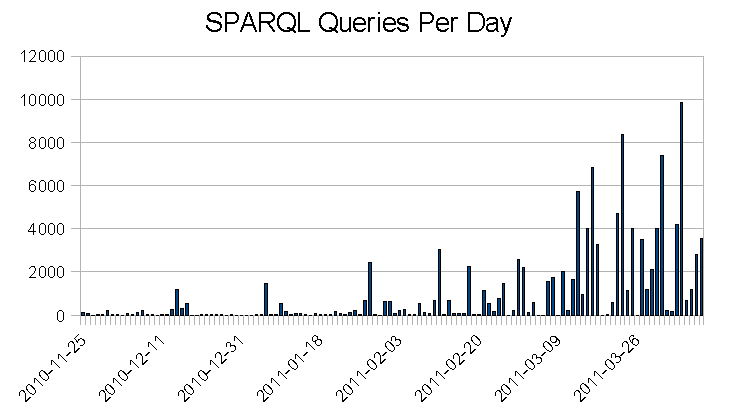
\includegraphics[width=0.5\textwidth]{images/SparqlQueriesPerDay.pdf}
%		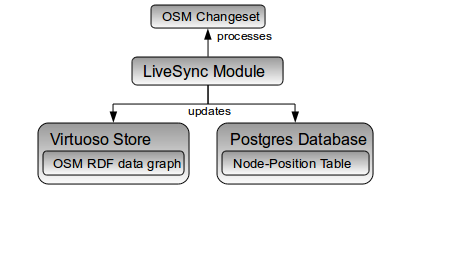
\includegraphics[width=0.4\textwidth]{images/LiveSyncArchitecture.png}
	\caption{Usage of the SPARQL endpoints.}
	\label{fig:sparql-queries-per-day}
\end{figure}
The diagram indicates that the LGD service is being actively used, and
that the usage rate is increasing.
%However, whether the high query counts towards the end remains at that level
%is yet to be evaluated.
%are one-shot or
%continuous uses need yet to be evaluated.

The current LGD release dataset contains about 65 million triples corresponding to
about 6.3 million nodes and 66 million triples corresponding to 7.1 million ways.
Table~\ref{tab:instance-counts} gives an overview of selected instance
counts in the static SPARQL endpoint, and their increase in number in LGD live
one after processing changsets corresponding to roughly three weeks.
\begin{table}[hb]
\begin{tabular}{lrr}
\toprule
class				&\#instances (static) & \#instances (live) \\
\midrule
Ways					&\val{7132373} &\val{7334925} \\
Nodes					&\val{6251067} &\val{7022481} \\
\midrule
Stream						&\val{2377952}	&\val{2419467} \\
Parking					&\val{520901} &\val{537477} \\
Village					&\val{516547} &\val{522570} \\
Shop					&\val{497820} &\val{519164} \\
Hamlet						&\val{415609} &\val{424179}\\
School				&\val{361239} &\val{366070} \\
PlaceOfWorship						&\val{359563} &\val{363225}\\
Restaurant &\val{173350} &\val{177888}\\
FastFood					&\val{67980} &\val{69772}\\
Pub 					&\val{67279} &\val{68279}\\
\bottomrule
\end{tabular}
\caption{Comparison of data from April 6th with live data from April 30th 2011.}
\label{tab:instance-counts}
\end{table}

Regarding LGD live sync performance, we measured the following values: on
average, the processing time of a single minutely OSM changeset takes 5 seconds with our filter configuration.
Between April 6 and April 30, about 40\,000 changesets were processed, each of them corresponding to an average addition of 620 and removal of 42 triples affecting 102 distinct resources.
%Evaluating 40K minutely changesets, each of them corresponds to
%an average addition of 620, and removal of 42 triples; affecting an average of
%102 distinct resources.

In the initial LGD release of 2009, there were 50 object properties.
However most of them were considered to be better suited as classes, resulting
in the relatively low number of only 9 object properties in the current
release.




%\begin{table}[htb]
%\renewcommand{\tabcolsep}{5pt}
%\begin{tabularx}{\textwidth}
%{
%>{\hsize=\hsize }L 
%>{\hsize=\hsize }L 
%>{\hsize=\hsize }L
%>{\hsize=\hsize }L 
%>{\hsize=\hsize }L 
%>{\hsize=\hsize }L 
%}
% \toprule
% \textbf{Interface}   &
% \textbf{Usage count} &
% \textbf{Avg. Time}   & 
% \textbf{P 1s}  & 
% \textbf{P 5s}  &
% \textbf{P 10s} & 
%\\
%\midrule
%Rest, Local-DB    &  5000 &   3   &    50\% &    50\% &    50\%  \\
%\midrule
%Rest, Osm-Wrapper &     - &   3   &    50\% &    50\% &    50\%  \\
%\midrule
%Sparql, Static    &  3000 &   3   &    50\% &    50\% &    50\%  \\
%\midrule
%Sparql, Live      &   100 &   3   &    50\% &    50\% &    50\%  \\
%\bottomrule
%\end{tabularx}
%\caption{Interface Performance Statistics}
%\label{tab:ips}
%\end{table}
%P-xs: What fraction of the queries could be answered within x seconds.
%Probably plot this as a graph, once we have that data.



\section{Tools using LinkedGeoData}
\label{sec:applications}

\begin{figure*}[tb]
	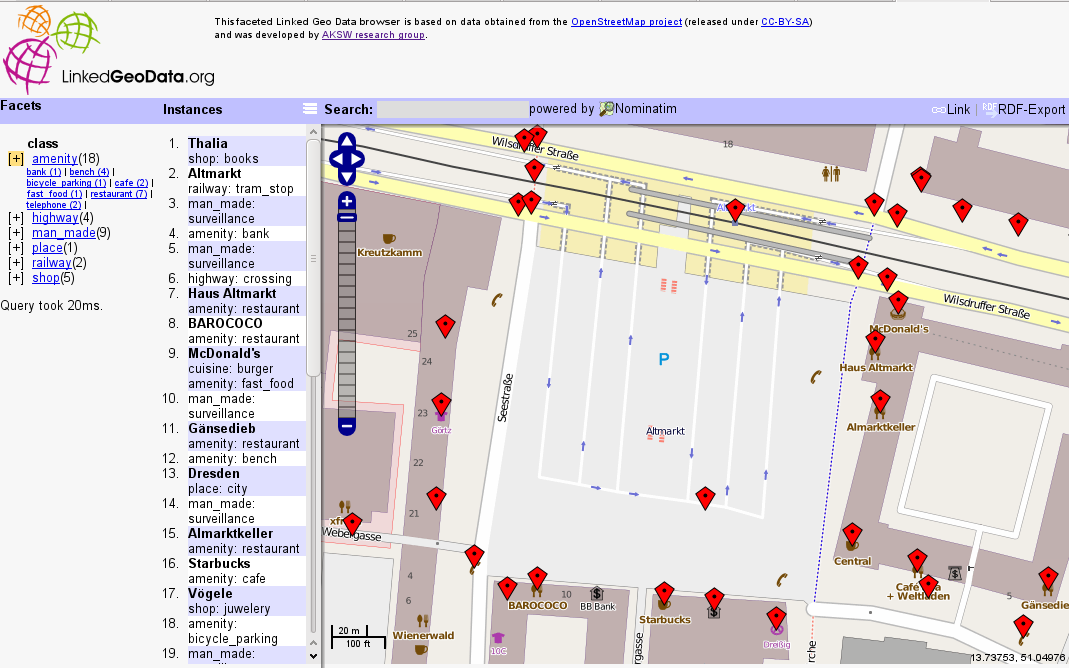
\includegraphics[width=.85\textwidth]{images/LGDBrowser}
	\caption{LinkedGeoData Browser.}
	\label{fig:browser}
\end{figure*}

\subsection{LGD Browser}
% JL: Browserbeschreibung ist teilweise aus dem ISWC-Paper uebernommen

In order to showcase the benefits of revealing the structured information in OSM,
we developed a facet-based browser and editor for
LinkedGeoData (see Figure~\ref{fig:browser})\footnote{Available online at: \url{http://browser.linkedgeodata.org}}.
It allows to browse the world by using a
``slippy map''\footnote{\url{http://wiki.openstreetmap.org/wiki/Slippy_Map}}.
Once a region is selected, the browser analyzes the descriptions of nodes and ways in that region and generates facets for filtering. Once a facet or a specific facet value has been
selected, matching elements are displayed as markers on the map and in a list.
If the selected region is changed, these are updated accordingly.

Performing the facet analysis naively, i.e. counting properties and property values
for a certain region, becomes slower the greater the size of 
the search region. This is due to the fact that the database has to
aggregate the facets from all the entities that fall into the search region.

To resolve this problem we precomputed tile-based statistics at various zoom
levels. If zoomed in close, the exact counts will be
measured, however if zoomed out the counts will be approximated by aggregating
the the statistics of the visible tiles.

Furthermore, there are several new smaller LGD browser features compared to its previous version described in~\cite{linkedgeodata}. For instance, an RDF export of the current map selection including its facets can now be performed.
This allows the easy extraction of a relevant fragment of LinkedGeoData for use
within other tools. For each point on the map, its RDF source can be retrieved and it can be edited on OpenStreetMap. The browser has been extended by a search function powered by \emph{OpenStreetMap Nominatum}. The facet support has been extended to object properties, i.e.~values of those properties can now be restricted in the facet selection. Finally, the LGD browser now provides a permanent link feature.

%Currently the tile ids are assigned according to the z-curve\todo{ref}
%numbering. This results in adjacent tiles having mostly a
%small difference between their ids. For this reason, lookups for tiles in an
%area This property results in which accounts for for efficient lookups


%Whether using 
 
%  tile ids are integers values that are assigned according to
% the
%z-curve\todo{ref} numbering. This results in adjacent tiles having mostly a
%small difference between their ids.  which accounts for for efficient lookups
%Whether using 

% can only use either the
%longitude or the latitude index. Combining both \-- longitude and latitude \--
%in one index is also impossible, since, given a certain latitude region, only
%elements in a relatively small longitude region are sought for.

%switch between two lookup strategies depending on the zoom level:
%When zoomed in close, the search region is small, and we perform the query
%query based on the nodes' positions. The postitions are indexed using 
%postgis' r-tree index.
%For each tile-id we then store the number of occurrences of the tags in it.
%When the user browses to a certain region, the application has to determine
%all the tiles intersecting that region.
%Since co-located tiles are assigned to adjacent tile ids, a certain region
%usually consists of a small number of tile ranges, which can be efficiently
%processed by the DBMS.


%\todo{Ok, This section drifted from reality, and now i broke it.}
%For computing the facets when zoomed out, we keep statistic tables that work
%as follows: At each zoom level, the map is divided into tiles, whereas the
%tiles are assigned ids according to the
%z-curve~\cite{zcurve}\footnote{Sometimes referred to as quadtile by the OSM
%community, see \url{http://wiki.openstreetmap.org/wiki/QuadTiles}} numbering.
%The consequence of the numbering is, that the ids of adjacent tiles are
%relatively close to each other, enabling efficient query evaluation with a
%B-Tree index. Note that   


%Even these indexing optimizations were not yet sufficient to obtain acceptable
%response times for the faceted browser. In order to further increase the
%querying performance, we precomputed the counts for all properties on all
%tiles, as well as the counts of all property values for a set of predefined
%properties of which we know that they have only a limited number of values.
%We did that not only for the highest zoom level, but for each zoom level which
%users are able to select. The lower the zoom level, the more the number of
%tiles reduces and the faster corresponding property and property value count
%aggregates can be computed.


\subsection{STEVIE}

STEVIE~\footnote{\url{http://tiny.cc/stevie10}}~\cite{stevie} is an application
developed by the Institute for Web Science and Technologies at the University of
Koblenz, which uses LinkedGeoData.
STEVIE allows one to create and edit points of interests (POIs)~(see
Figure~\ref{fig:stevie}) and annotate them semantically. The annotations use the LinkedGeoData ontology and are also interlinked to DBpedia. The annotations allow to employ clustering techniques in STEVIE, which are used to group sets of similar objects within the limited screen size of a mobile phone. The application allows the creation of events and, therefore, combines spatial and temporal information. An emphasis is put on providing an intuitive user interface for navigating those two dimensions. In order to display POIs and classify them, STEVIE uses the LinkedGeoData REST interface, ontology and SPARQL endpoint.

\begin{figure}[bt]
	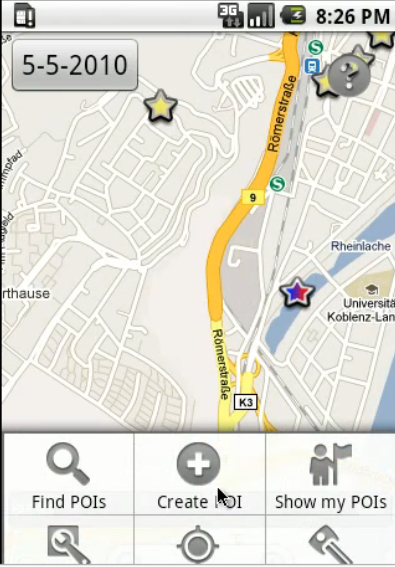
\includegraphics[width=.35\textwidth]{images/stevie}
	\caption{Creation of a point of interest in STEVIE. The application includes a temporal dimension and highlights POIs where events take place in the selected time span.}
	\label{fig:stevie}
\end{figure}

\subsection{BeAware}

BeAware\footnote{\url{http://beaware.at/}} is a website, which enables one
to manage events and integrates them with geographic information. It
uses its own ontology for events and integrates LinkedGeoData for choosing locations. In particular, the curated ontology of LinkedGeoData provides benefits for the application\footnote{\url{http://alexidsa-en.blogspot.com/2010/06/rdf-vs-nonrdf-for-geodata-at-beaware.html}}: ``First of all, LinkedGeoData ontology that connects all OpenStreetMap categories and properties excellently suits our interface of new place choosing (in addition, it allows to use inference engine, for example, for retrieving buildings of all types).'' Figure~\ref{fig:beaware} shows a screenshot for choosing the location of an event. An advantage gained by this association is that it facilitates querying for events at a particular location or within a particular city. In addition, in some cases further information about the location from an interlinked data source is available and can be presented to the user.

\begin{figure*}[htb]
	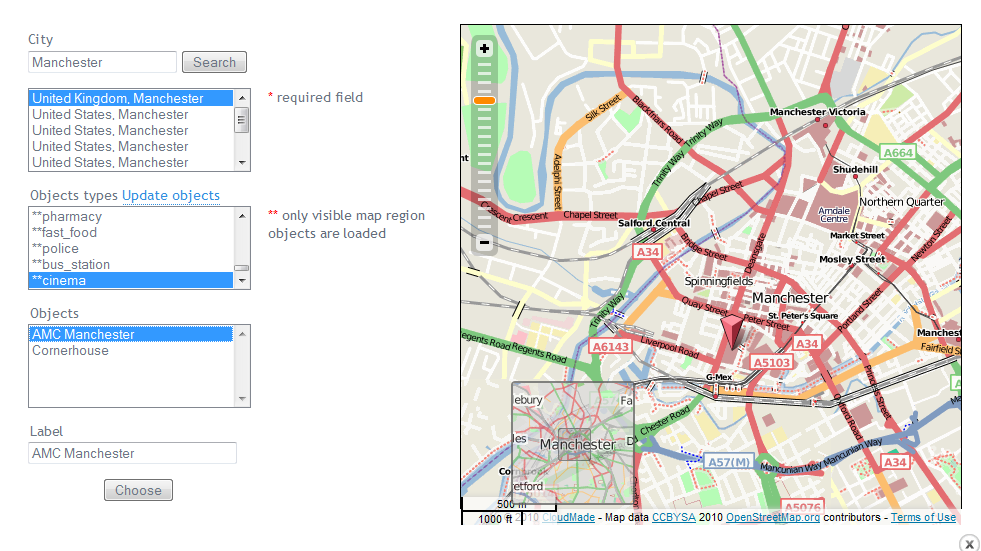
\includegraphics[width=.85\textwidth]{images/BeAware1}
	\caption{Marking the location of an event in BeAware.}
	\label{fig:beaware}
\end{figure*}

\subsection{Layar}

Layar\footnote{\url{http://www.layar.com}} is an augmented reality browser for mobile phones. Within Layar, a LinkedGeoData layer was developed. This allows to view the surrounding objects of a person via the mobile phone camera. The LinkedGeoData ontology is used to classify objects and map them to displayed icons. The layer uses \verb|rdfs:label|, which is aggregated from several tags in OpenStreetMap, to display the name of an object. Further triples describing an object are show in a detail view.

\begin{figure}
	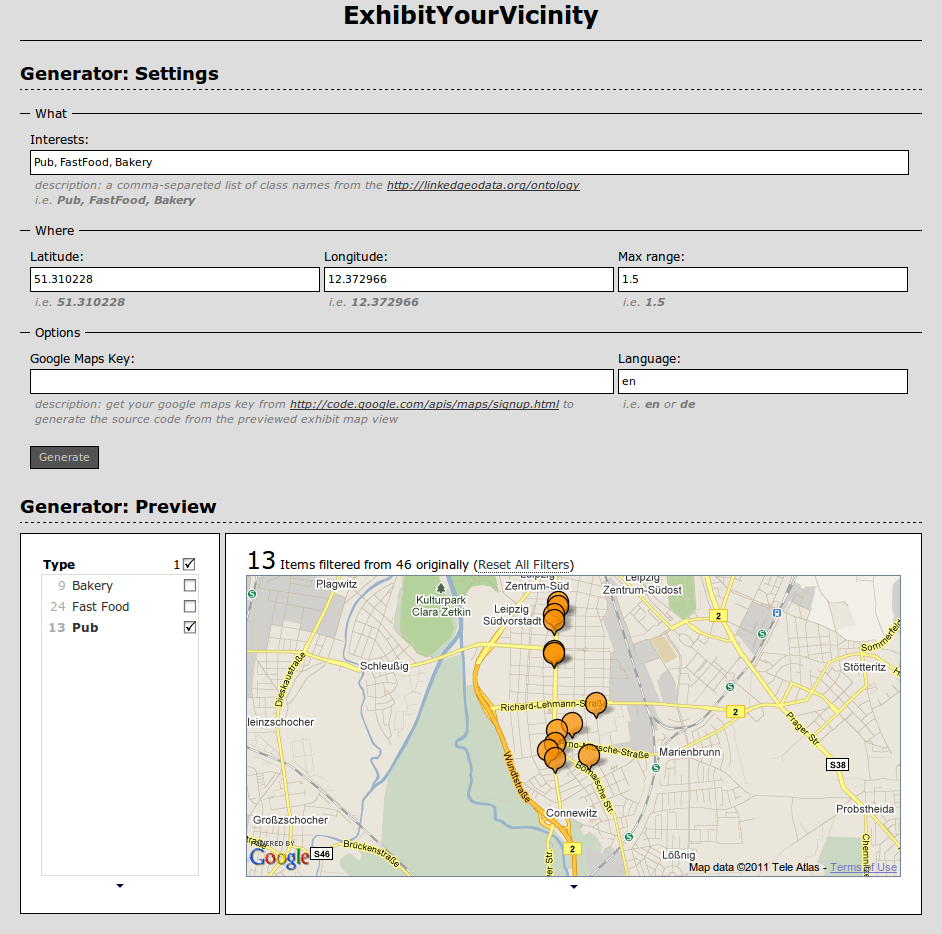
\includegraphics[width=.45\textwidth]{images/vicibit}
	\caption{Vicibit is a tool to generate custom views on LinkedGeoData via Exhibit. The example shows a faceted view on nearby pubs, bakeries and shops. The code generated by Vicibit can easy be pasted into blogs, forums and web pages.}
	\label{fig:vicibit}
\end{figure}

\subsection{Vicibit}

Vicibit\footnote{\url{http://vicibit.linkedgeodata.org}} (``exhibit your vicinity'') is a tool working on top of LinkedGeoData Live, which allows to create customised views on LinkedGeoData.
It enables users to pick classes from the LinkedGeoData ontology they are
interested in as well as a default map section, which should be displayed. The tool then generates HTML code, which creates a map displaying all items belonging to the selected classes as well as the ability to filter by facets. Technically, this is realised by applying the Exhibit framework\footnote{\url{http://www.simile-widgets.org/exhibit/}} on data in the LinkedGeoData Live SPARQL endpoint. A typical use case is that a webpage or blog entry describing a particular event can be enriched with a map of nearby pubs and other shops (see Figure~\ref{fig:vicibit}).



\section{Related Work}
\label{sec:related}

We split the presentation related work into five parts: 
First, we describe initiatives for integrating spatial information in the Web of Data. 
Afterwards, we summarize work on techniques for converting relational databases to RDF,
which is a crucial task we faced in LinkedGeoData. 
We then give an overview of triple stores supporting geographic data more complex than
point data. Finally, we review some related work done by the GIS community, give
pointers to interlinking frameworks and explain our choice of using SILK and LIMES.
 % and conclude with other related work, which we deem important, but does not fall into the three previous categories.

\subsection{Spatial RDF Datasets}

In the following, we describe spatial data sets, which are available as RDF and we consider important.

\begin{description}
\item \emph{Ordnance Survey}\footnote{\url{http://www.ordnancesurvey.co.uk}} is the national mapping agency in Great Britain. 
Over the past years, they released some of their products as Linked Data\footnote{\url{http://data.ordnancesurvey.co.uk}}. 
Ordnance Survey provides very accurate, high-quality data and represents a major contribution to the spatial data web. 
In a comparison between Ordnance Survey data~\cite{osm_ordnance_survey} focused on England and London in particular, OSM data was, however, also fairly accurate. 
A main difference between both efforts is that OpenStreetMap, and thereby also LinkedGeoData, are world-wide and community-driven approaches.
\item \emph{GeoNames} is a comprehensive global spatial database containing several million
features, such as cites, forests, and peaks.
This data has been converted to RDF\footnote{\url{http://www.geonames.org/ontology/}} and is served as Linked Data.
GeoNames provides RDF properties for navigating spatial hierarchies (parent/child), publishes postal codes, labels, population figures, type information (via feature codes) and other properties of spatial entities. 
Due to this wealth of information, we developed a fine-grained interlinking between LinkedGeoData and GeoNames as described in Section~\ref{sec:interlinking}. 
A difference between GeoNames and OpenStreetMap is that OSM allows free tags, which makes it easier to extend and tailor for new, previously unforeseen usage scenarios.
For instance, shops in OSM sometimes (specifically 60 thousand times as of April 2011) contain opening hours.
Another example is the wheelchair tag, used 24 thousand times, which indicates whether or not a spatial entity is accessible via a wheel chair. 
OpenStreetMap also has a larger community than GeoNames with several hundred thousand users and more fine-grained data, which even includes entities such as traffic lights or trash bins.
\item The \emph{United Nations FAO (Food and Agriculture Organisation) Geopolitical Data}~\cite{un_fao} provides RDF descriptions of countries and other political units as well as relations between them. 
While it contains only a small number of instances (298 in May 2011), it includes very detailed information on those instances. 
For this reason, we decided to provide interlinks with UN FAO.
% \todo{Jens: I looked at the data and in my opinion it would be easy and worthwhile to interlink it with LinkedGeoData countries (needs only a single SILK/LIMES spec.} => almost done
\item \emph{GeoLinkedData.es} is an open initiative to provide Spanish geospatial data~\cite{geolinkeddata}. 
It focuses on hydrography features and integrates several existing data sources.
\item \emph{NUTS (Nomenclature of Territorial Units for Statistics)} provides a hierarchical system for describing the economic territory of the European Union~\footnote{\url{http://epp.eurostat.ec.europa.eu/portal/page/portal/nuts_nomenclature/introduction}}. 
The NUTS hierarchy is established by EuroStat. EU NUTS data has been converted to RDF~\footnote{\url{http://rdfdata.eionet.europa.eu/ramon/nuts2008/}}. 
It allows to explore the hierarchy via Linked Data, e.g.~a possible path along the ``partOf'' property is  Inner London East $\to$ Inner London $\to$ London $\to$ UK.
\end{description}

\subsection{Relational Database to RDF Conversion and Mapping}

Converting relational databases to RDF is a significant area of research with several approaches published and many tools available. 
In particular, there is the W3C RDB2RDF working group, which aims to standardize a database to RDF mapping language~\cite{r2rml}. 
Instead of providing an in-depth overview, we refer to recent surveys~\cite{RDB2RDF,SWJ_RDB2RDF}  and overviews\footnote{\url{http://esw.w3.org/topic/Rdb2RdfXG/StateOfTheArt}} on this topic.
%\url{http://esw.w3.org/topic/Rdb2RdfXG/StateOfTheArt}
%\url{http://www.w3.org/2005/Incubator/rdb2rdf/RDB2RDF_SurveyReport.pdf}
%\url{http://www.semantic-web-journal.net/content/bringing-relational-databases-semantic-web-survey}
There are various tools available implementing the surveyed approaches such as D2R, Triplify, DartGrid, DataMaster, MapOnto, METAmorphoses, ODEMapster, RDBToOnto, RDOTE, Virtuoso RDF Views and VisAVis. 
For LinkedGeoData, we decided to use a custom mapping solution as described in Section~\ref{sec:rdf_mapping}, despite the number of available conversion tools. 
The reason for this choice was the particular tag structure of OSM, which allows us to provide a highly flexible schema as well as handle a very high amount of data via our approach.
% This way, a live synchronisation with OpenStreetMap is feasible.


%reviewt drei Gezetteere (GeoNames, Getty, und ADL)
%  und diskutiert design entscheidungen und implementation einer OWL
%  Ontologie, wie sie auch für similarity searches verwendbar ist.

%Implementations of 
% gibt eine ausführliche diskussion über such
%paradigmen (intensional, extensional, hybrid) in bezug auf von SIM-DL, eine
%similarity theorie für beschreibungslogiken, und diskutiert eine architektur,
%um SIM-DL in SDI (spatial data infrastructure) zu integrieren.

% (Spatially-Aware Information Retrieval on the
% Internet) SPIRIT\cite{intelligent_spatial_search} ist eine (wenn nicht
% velleicht damals die) weitere spatially aware suchmaschine.
  
%research topics bei solchen such engines sind:
%grounding (lokalisierung), disambiguierung, query expansion (z.B. semantisches
%anreichern von queries), ranking, fuzzy spatial relations (``near'')
  
  
\subsection{Triple Stores supporting Complex Geometries}
\label{sec:geo-semantic-web}

In the relational database realm, support for complex geometric data
(points, lines, and polygons) is already well established. Examples are
MySQL\footnote{\url{http://www.mysql.com}},
PostgreSQL\footnote{\url{http://www.postgresql.org/}}, and
Oracle\footnote{\url{http://www.oracle.com}}.
Meanwhile, in the Semantic Web, the support for geometric data has also
increased significantly. Currently, we are aware of four triple stores
supporting this kind of data:
\emph{OWLIM Standard Edition}\footnote{\url{http://www.ontotext.com/owlim/geo-spatial}}
(OWLIM-SE, previously known as BigOWLIM),
\emph{Open Sahara}\footnote{\url{http://opensahara.com}},
\emph{Parliament}\footnote{\url{http://parliament.semwebcentral.org/}}, and
\emph{AllegroGraph}\footnote{\url{http://www.franz.com/agraph/allegrograph/}}. 

So far there has not been a standard query language for geospatial
data in the Semantic Web. GeoSPARQL is a proposed extension to
SPARQL~{1.0}~\cite{sparql} with the aim to provide this functionality.
It is currently at the stage of becoming a standard by the Open Geospatial consortium\footnote{\url{http://www.opengeospatial.org/}}.   
With these tools, tasks that require complex operations on geometries
become possible in the Semantic Web.
%  This effort can be expected to eventually become supported by RDB-RDF mapping solutions.
% \todo{ideally add the post office
%use case if I ever find this paper again (Something along the lines of Peter
%met Sarah across the street at the post office. System plots likelyhood of
%where they met.)}
  
We chose Virtuoso as the backend for LinkedGeoData because of its good
performance~\cite{BerlinSparql} and our assumption that point geometries
would be sufficient for most of our interlinking tasks. Although this turned
out to be true, in the future we want to extend these tasks to complex
geometries and therefore also evaluate the other stores.

\subsection{Gazetteer Mapping}

Our interlinking approach is very similar to the matching of gazetteers in
traditional Geographic Information Systems (GIS): \cite{gazetteer_core_elements}
discusses the alignment of two major gazetteers. For this
purpose, place names, types and footprints (geographical entities such as
point, lines and polygons) were identified as the most fundamental features of gazetteers.
These entities closely resemble the concepts of classes, labels and
geometries, on which we based our interlinking.
Prior work about the derivation of an OWL ontology suitable for similarity
searches from gazetteers is given in \cite{gazetteer_ontology}. 
A comprehensive discussion about similarity search paradigms
for Description Logics is lead in \cite{sim_ir}.

\subsection{Interlinking and Ontology Mapping}

There have been several decades of research starting with the integration of
different database schemata. Tools like COMA~\cite{coma} provide rich support
for various matching operations between databases as well as between RDF
knowledge bases. \cite{BraunerIFC07}~describes a semantic approach for matching
export schemas of geographical database Web services, based on the use of a
small set of typical instances. The paper also contains an extensive
experiment, carried out within the context of two gazetteers, GeoNames and the
ADL gazetteer, to illustrate the idea. \cite{conf/icdim/ManguinhasMB08}
describes an approach integrating spatial data from multiple sources, which also
incorporates a temporal dimension. For interlinking LinkedGeoData, we mainly
searched for instance matching tools, since our main goal is to match specific
points of interests in different knowledge bases. In this area,
SILK and LIMES are the most widely used applications. We extended
SILK with an appropriate metric for matchings based on WGS84 distance between
points, which was later included in the official SILK release. A main benefit
for SILK as well as LIMES, which we both use, is their ability to handle large
volumes of data and use SPARQL endpoints as input source.

\begin{comment}
\url{http://de.wikipedia.org/wiki/Web\_Map\_Service}
\url{http://de.wikipedia.org/wiki/Web\_Feature\_Service}

Analysis of edit behaviour:
"Annotating Spatial Features in OpenStreetMap"

Current work in the area of spatio temporal data can be roughly classified
into RDF-Conversion, Interlinking, RDB-RDF mapping and ontology engineering,
(whats more?) \todo{what else}.

Workshop On Linked Spatiotemporal Data 2010
   \url{http://stko.psu.edu/lstd2010/}

Thing the people from the NeoGeoVocabCamp are working on
    GeoLinkedData
g2r
d2g

Das ist das tolle Dokument:
\url{http://linkeddata.com.ar/doc/2011/03/note.html}
\end{comment}

\section{Conclusions and Future Work}
\label{sec:conclusions}

The transformation and publication of the OpenStreetMap data according to the
Linked Data principles adds a new dimension to the Data Web: spatial data can
be retrieved and interlinked on an unprecedented level of granularity. These
enhancements may further contribute to semantic-spatial search engines, such as
~\cite{sim_ir, spirit}, and enable a variety of new Linked Data applications such
as geo-data syndication (publishing information about geographical entities via
feeds). Another example is personalized and context-sensitive
spatial Linked Data update propagation and consumption, which might be
realized with systems such as sparqlPuSH~\cite{sparql_push}.
 

The dynamics of the OpenStreetMap project will
ensure a steady growth of the LinkedGeoData dataset. Furthermore, we established mappings with DBpedia and GeoNames as the central interlinking hubs for spatial information on the Web of Data.
Despite the recent advances in RDF data management, it became clear during our work on LinkedGeoData that spatial data of the size of OpenStreetMap still poses a major challenge wrt. scalability.
Substantial engineering effort was required to optimize the performance of the querying interfaces, live synchronisation as well as the interlinking.

Currently, our transformation approach imposes the following\emph{ limitations} on the use of
LinkedGeoData:
\begin{itemize}
  \item The current \emph{ontology} is mainly automatically derived from
  OpenStreetMap tags, with mostly just minor manual edits. However, it could
  benefit from axiomatizations, such that, for example, any \emph{PlaceOfWorship} with religion
  \emph{christian} is a \emph{Church}.
  The extent to which the addition of disjointness axioms makes sense needs yet
  to be investigated. For instance, currently instances corresponding to
  hotels that also offer a restaurant are currently tagged with both types.
  However, an alternative solution would be to model such instance as a
  \emph{Hotel}, that offers a feature that is a \emph{Restaurant}. For these
  kinds of design decisions, we envision a solution similar to the \emph{DBpedia
  Mapping Wiki}\footnote{\url{http://mappings.dbpedia.org}}, that enables the
  community to contribute to the axiomatization of the ontology.
  
  \item Our \emph{filtering} (see Section~\ref{sec:filtering}) currently
  discards a significant amount of data from OSM. Hence, there are use
  cases that are possible with OSM data, but not with LinkedGeoData yet.
  For example, since we filter out ways with more than 20 nodes, 
  routing\footnote{\url{http://wiki.openstreetmap.org/wiki/Routing}} is currently not
  possible based on the LinkedGeoData SPARQL endpoints.
    
  \item Because we do not support OpenStreetMap relations yet, information about
  compound entities is also not yet available in LinkedGeoData. 
  Examples of such entities are: multipolygons (collections
  of polygons, where each member may act either as solid or as a hole), or
  designation signs. Further examples include large boundaries, waterways, and
  routes, that are modelled with way segments.
\end{itemize}

As for the latter two limitations, we are currently investigating whether and
how these limitations can be overcome by directly rewriting SPARQL queries to SQL queries over
the relational schema of OpenStreetMap.
Although substantial progress was made in RDB-RDF mapping
during the last years, and implementations are now more robust, scalability
and the lack of support for geometry datatypes is still an issue
preventing a direct deployment of these technologies for LinkedGeoData.

Another stream of future work is the better support for geometries according to
the current NeoGeoVocabulary
development\footnote{\url{http://geovocab.org/doc/neogeo.html}}, which we are
supporting. A semantic misrepresentation currently found in LinkedGeoData, for
example, is the missing separation of geometries (such as points and polygons)
and features (such as hotels and pubs), which we plan to resolve in the future.
%In the future, we plan to implement thi
%plan to attach geometries to entities, i.e. points of interest, instead of
%identifying both.

Finally, we identified further candidates that seem worthwhile for interlinking:
\begin{itemize}
\item The \emph{CIA World
Factbook}\footnote{\url{https://www.cia.gov/library/publications/the-world-factbook/}}
contains detailed information on the country level, such as their conventional
names, their birthrate, and their gross domestic product. An RDF version is
hosted by the Free University of
Berlin\footnote{\url{http://www4.wiwiss.fu-berlin.de/factbook/}}.

\item The site \url{climb.dataincubator.org} hosts a collection of data of about
{1400} climbing locations with latitude/longitude information. The resources
were collected from various climbing web sites and converted to RDF.

\item \emph{Last.fm}\footnote{\url{http://last.fm}} has information about music
artists, as well as events, such as performances and festivals. Many event locations are
geo-tagged, making them suitable candidates for interlinking.
There exist at least two wrappers for the {last.fm} API that return
RDF\footnote{\url{dbtune.org/last-fm/} and \url{lastfm.rdfize.com/}}.

\end{itemize}



%\section*{Acknowledgments}
%We would like to thank OpenLink for providing an enterprise
%edition of the Virtuoso database system that offers support for spatial SPARQL
%queries. Furthermore, the authors thank the members of the LinkedGeoData
%community and 3rd party application developers for their valuable feedback and contributions to the project.
%In particular, we would like to mention Robert Schulze for his work on Vicibit.
%This work was supported by a grant from the European Union's 7th Framework
%Programme provided for the projects LOD2 (GA no. 257943) and LATC (GA no. 256975).

%%%%%%%%%%% The bibliography starts:
%\bibliographystyle{abbrv}
%\bibliography{swj_linkedgeodata,../../bib/aksw}

%\appendix

\section{Prefixes Used}
\label{sec:prefixes}

The following prefixes are used in the paper:

\begin{ttfamily}
\begin{lstlisting}[language=SQL,basicstyle=\scriptsize,numbers=left,numberstyle=\tiny,breaklines=true,breakindent=0cm,breakautoindent=false,morekeywords={OPTIONAL,FILTER}]
lgd:    http://linkedgeodata.org/triplify/
lgdo:    http://linkedgeodata.org/ontology/
wgs84:   http://www.w3.org/2003/01/geo/wgs84_pos#
foa:     http://www.fao.org/countryprofiles/geoinfo/geopolitical/resource/
dbpedia:  http://dbpedia.org/resource/
rdf:      http://www.w3.org/1999/02/22-rdf-syntax-ns#
rdfs:     http://www.w3.org/2000/01/rdf-schema#
owl:      http://www.w3.org/2002/07/owl#
xsd:      http://www.w3.org/2001/XMLSchema#
georss:   http://www.georss.org/georss/
\end{lstlisting}
\end{ttfamily}

%\end{document}

